\chapter{Fairness Influence Functions}
%\section{Societal Impact}
%In this paper, we quantify the influence of input features on the incurred bias/unfairness of the classifier on a dataset. This quantification facilitates our understanding of potential features or subsets of features attributing highly to the bias. This also allows us to understand the effect of the fairness enhancing algorithms in removing bias and their achievement/failure to do so. To the best of our understanding, this paper does not have any negative societal impact. 


\begin{comment}
\section{FIF as Difference of Conditional Variances: Proof of Theorem 1}\label{fairness_fairXplainer_sec:proof_1}

\begin{reptheorem}{lemma:fif_rep}[FIF as Difference of Conditional Variances]
	Let $ V_{\mathbf{a}, \mathbf{S}} \triangleq \mathsf{Var}_{\nonsensitive_{\mathbf{S}}}[\widehat{Y} = 1|\sensitive = \mathbf{a}] $ be the decomposed conditional variance of the classifier's positive prediction for the sensitive group $ \sensitive = \mathbf{a} $, where features $ \nonsensitive_{\mathbf{S}} $ are jointly varied. Let $\mathbf{a}_{\max}$ and $\mathbf{a}_{\min}$ be the most and the least favored groups, respectively. Then, FIF of $ \nonsensitive_{\mathbf{S}} $ corresponding to statistical parity is
	\begin{equation}\tag{\ref{fairness_fairXplainer_eq:fif_decompose}}
	w_{\mathbf{S}}  = \frac{V_{\mathbf{a}_{\max},\mathbf{S}} - V_{\mathbf{a}_{\min},\mathbf{S}}}{1 - (\Pr[\widehat{Y} = 1 |  \sensitive = \mathbf{a}_{\max}] + \Pr[\widehat{Y} = 1 |  \sensitive = \mathbf{a}_{\min}])},
	\end{equation}
	and FIFs defined by Equation~\eqref{fairness_fairXplainer_eq:fif_decompose} satisfy Axiom~\ref{fairness_fairXplainer_axm:additivity}.
\end{reptheorem}


\begin{proof}

Let $ B_{\mathbf{a}} \in \{0, 1\} $ be a Bernoulli random variable such that $ B_{\mathbf{a}} = 1 $ denotes the classifier predicting positive class $ \hat{Y} = 1 $ for an individual belonging to the sensitive group $ \sensitive = \mathbf{a} $, and $ B_{\mathbf{a}} = 0 $ denotes $ \hat{Y} = 0 $. Hence, if $ p_\mathbf{a} \triangleq \Pr[B_\mathbf{a} = 1] $, then $ p_\mathbf{a} $ is also the conditional probability of positive prediction of the classifier,  $ p_\mathbf{a} = \Pr[\hat{Y} = 1 |  \sensitive = \mathbf{a}] $. The variance of $ B_{\mathbf{a}} $ is computed as
\begin{align*}
	\mathsf{Var}[B_\mathbf{a}] = p_{\mathbf{a}}(1 - p_{\mathbf{a}}). 
\end{align*}

Now, we consider two Bernoulli random variables $ B_\mathbf{a} $ and $ B_\mathbf{a'} $ associated with two different sensitive groups $ \sensitive = \mathbf{a} $ and $ \sensitive = \mathbf{a}' $, respectively. The difference in variances between $ B_\mathbf{a} $ and $ B_\mathbf{a'} $ implies that
\begin{align*}
	\mathsf{Var}[B_\mathbf{a}] - \mathsf{Var}[B_\mathbf{a'}] &= p_{\mathbf{a}}(1 - p_{\mathbf{a}}) - p_{\mathbf{a'}}(1 - p_{\mathbf{a'}}) \\
	&= p_{\mathbf{a}} - p_{\mathbf{a}}^2 - p_{\mathbf{a'}} + p_{\mathbf{a'}}^2 \\ 
	&= (p_\mathbf{a} -  p_\mathbf{a'}) (1 - (p_\mathbf{a} + p_\mathbf{a'}))
\end{align*}

After reorganization, we express the difference in probabilities $ p_\mathbf{a} -  p_\mathbf{a'} $ as
\begin{align}
	\label{fairness_fairXplainer_eq:sp_to_var}
	p_\mathbf{a} -  p_\mathbf{a'}  = \frac{	\mathsf{Var}[B_\mathbf{a}] - \mathsf{Var}[B_\mathbf{a'}]}{1 - (p_\mathbf{a} + p_\mathbf{a'})}
\end{align}




By setting $ \mathbf{a} = \mathbf{a}_{\max} $ and $ \mathbf{a'} = \mathbf{a}_{\min} $ in Equation~\eqref{fairness_fairXplainer_eq:sp_to_var}, we express the statistical parity of the classifier in terms of the scaled difference in the conditional variance of the positive prediction of the classifier. 
\begin{align}
	f_{\mathsf{SP}}(\alg, \mathbf{D}) \triangleq p_{\mathbf{a}_{\max}} -  ~~p_{\mathbf{a}_{\min}}  &= \frac{	\mathsf{Var}[B_{\mathbf{a}_{\max}}] - \mathsf{Var}[B_{\mathbf{a}_{\min}}]}{1 - (p_{\mathbf{a}_{\max}} + p_{\mathbf{a}_{\min}})}\label{fairness_fairXplainer_eq:sp_var_diff}\\
	&= \frac{	\mathsf{Var}[\hat{Y} = 1| \sensitive = \mathbf{a}_{\max}] - \mathsf{Var}[\hat{Y} = 1| \sensitive = \mathbf{a}_{\min}]}{1 - (p_{\mathbf{a}_{\max}} + p_{\mathbf{a}_{\min}})} \notag.
\end{align}

%The last inequality is obtained by the definition of $B_{\mathbf{a}}$.

Next, we apply variance decomposition (Equation~\eqref{fairness_fairXplainer_eq:variance_decomposition_set_notation}) to estimate the influence of each $ \nonsensitive_{\mathbf{S}} $. From Equation~\eqref{fairness_fairXplainer_eq:variance_decomposition_set_notation} in Section~\ref{fairness_fairXplainer_sec:preliminaries}, we obtain that the variance of $ B_{\mathbf{a}} $ can be decomposed as 
\[ \mathsf{Var}[B_\mathbf{a}] = \sum_{\mathbf{S} \subseteq [\numnonsensitive] \setminus \emptyset} V_{\mathbf{a}, \mathbf{S}},\] 
where $ V_{\mathbf{a}, \mathbf{S}} $ denotes the decomposed variance of $ B_\mathbf{a} $ w.r.t.\ the features $ \nonsensitive_{\mathbf{S}} $ conditioned on the sensitive group $ \sensitive = \mathbf{a} $. 

Now, we apply variance decomposition on both $ \mathsf{Var}[B_{\mathbf{a}_{\max}}] $ and $ \mathsf{Var}[B_{\mathbf{a}_{\min}}] $ in Equation~\ref{fairness_fairXplainer_eq:sp_var_diff} to obtain

\begin{align}
f_{\mathsf{SP}}(\alg, \mathbf{D}) & = \frac{\mathsf{Var}[B_{\mathbf{a}_{\max}}] - \mathsf{Var}[B_{\mathbf{a}_{\min}}]}{1 - (p_{\mathbf{a}_{\max}} + p_{\mathbf{a}_{\max}})}= \sum_{\mathbf{S} \subseteq [\numnonsensitive] \setminus \emptyset} \frac{V_{\mathbf{a}_{\max}, \mathbf{S}} - V_{\mathbf{a}_{\min}, \mathbf{S}}}{1 - (p_{\mathbf{a}_{\max}} + p_{\mathbf{a}_{\min}})} \label{fairness_fairXplainer_eq:influence_value}
\end{align}
Finally, we estimate  the FIF of the subset of features $ \nonsensitive_{\mathbf{S}}  $ as 
\begin{align}
	w_{\mathbf{S}}  = \frac{V_{\mathbf{a}_{\max}, \mathbf{S}} - V_{\mathbf{a}_{\min}, \mathbf{S}}}{1 - (p_{\mathbf{a}_{\max}} + p_{\mathbf{a}_{\min}})}
\end{align} 
by separating the terms corresponding to $ \nonsensitive_{\mathbf{S}} $.

Following Equation~\eqref{fairness_fairXplainer_eq:influence_value}, $	w_{\mathbf{S}} $ satisfies Axiom~\ref{fairness_fairXplainer_axm:additivity} as $f_{\mathsf{SP}}(\alg, \mathbf{D}) = \sum_{\mathbf{S} \subseteq [\numnonsensitive] \setminus \emptyset} w_{\mathbf{S}} $.
\end{proof}

\end{comment}


\section{Proofs of Properties and Implications of FIF}
\begin{reptheorem}{fairness_fairXplainer_thm:fif_property}
	Let $ f(\alg, \mathbf{D}) $ be the bias/unfairness of the classifier $ \alg $ on dataset $ \mathbf{D} $ according to linear group fairness metrics such as statistical parity. Let $ w_{\mathbf{S}}  $ be the FIF of a subset of  features $ \feature_{\mathbf{S}} $ as defined in Eq.~\eqref{fairness_fairXplainer_eq:fif_decompose}. 
	\begin{enumerate}
		\item[(a)] \textit{The decomposability property} of FIF states that the sum of FIFs of all subset of  features is equal to the bias of the classifier. 
		\begin{align}
		\sum_{\mathbf{S} \subseteq [\numfeatures] } w_{\mathbf{S}} = f(\alg, \mathbf{D})
		\end{align}
		\item[(b)] \textit{The symmetry property} states that  two features $ Z_i $ and $ Z_j $ are equivalent based on FIF if the sum of corresponding individual influences and the intersectional influences with all other features are the same. Mathematically,
		\begin{align}
		\sum_{\mathbf{S}'' \subseteq [m]\setminus \{i,j\}}w_{\mathbf{S}''\cup \{i\}} = \sum_{\mathbf{S}'' \subseteq [m]\setminus\{i,j\}}w_{\mathbf{S}''\cup \{j\}}  
		\end{align}
		if $\sum_{\mathbf{S}' \subseteq \mathbf{S}\cup \{i\}} w_{\mathbf{S}'} = 		\sum_{\mathbf{S}' \subseteq \mathbf{S} \cup \{j\}} w_{\mathbf{S}'}$ for every non-empty subset $ \mathbf{S} $ of $ [\numfeatures] $ containing neither $ i $ nor $ j $. 
		\item[(c)] \textit{The null property} of FIF states that feature $ X_i $ is a dummy or neutral feature if sum of its individual influence and the intersectional influences with all other features is zero. Mathematically,
		\begin{align}
		\sum_{\mathbf{S}'' \subseteq [m]\setminus\{i\}}w_{\mathbf{S}''\cup \{i\}} = 0 	 
		\end{align}
		if	$\sum_{\mathbf{S}' \subseteq \mathbf{S} \cup \{i\}} w_{\mathbf{S}'} = 		\sum_{\mathbf{S}' \subseteq \mathbf{S}} w_{\mathbf{S}'}$ for every non-empty subset $ \mathbf{S} $ of $ [\numfeatures] $ that does not contain $ i $.
	\end{enumerate}
\end{reptheorem}



\begin{proof}
	(a) The decomposability property of FIF is based on GSA, where the total variance is decomposed to the variances of individual and intersectional inputs. 
	\begin{align*}
	\sum_{\mathbf{S} \subseteq [\numfeatures]} w_{\mathbf{S}} &= \sum_{\mathbf{S} \subseteq [\numfeatures]} \frac{V_{\mathbf{a}_{\max}, \mathbf{S}}}{ \Pr[\widehat{Y} = 0 \mid  \sensitive = \mathbf{a}_{\max}]} - \frac{V_{\mathbf{a}_{\min}, \mathbf{S}} }{\Pr[\widehat{Y} = 0 \mid  \sensitive = \mathbf{a}_{\min}]}\\
	&= \frac{\sum_{\mathbf{S} \subseteq [\numfeatures]} V_{\mathbf{a}_{\max}, \mathbf{S}}}{ \Pr[\widehat{Y} = 0 \mid  \sensitive = \mathbf{a}_{\max}]} - \frac{\sum_{\mathbf{S} \subseteq [\numfeatures]} V_{\mathbf{a}_{\min}, \mathbf{S}} }{\Pr[\widehat{Y} = 0 \mid  \sensitive = \mathbf{a}_{\min}]}\\
	&= \frac{V_{\mathbf{a}_{\max}}}{ \Pr[\widehat{Y} = 0 \mid  \sensitive = \mathbf{a}_{\max}]} - \frac{V_{\mathbf{a}_{\min}} }{\Pr[\widehat{Y} = 0 \mid  \sensitive = \mathbf{a}_{\min}]}\\
	&=\frac{\mathsf{Var}[\widehat{Y} = 1\mid\sensitive = \mathbf{a}_{\max}]}{\Pr[\widehat{Y} = 0 \mid  \sensitive = \mathbf{a}_{\max}]} - \frac{\mathsf{Var}[\widehat{Y} = 1\mid\sensitive = \mathbf{a}_{\min}] }{\Pr[\widehat{Y} = 0 \mid  \sensitive = \mathbf{a}_{\min}]}\\
	&= f_{\mathsf{SP}}(\alg, \mathbf{D})
	\end{align*}
	Thus, applying Lemma~\ref{fairness_fairXplainer_lm:sp_var_relation}, we prove the decomposability property of FIF for statistical parity.
	
	(c) We observe that 
	\begin{align}\label{fairness_fairXplainer_eq:sum_decomp}
		\sum_{\mathbf{S}' \subseteq \mathbf{S}\cup \{i\}} w_{\mathbf{S}'} = \sum_{\mathbf{S}' \subseteq \mathbf{S}} w_{\mathbf{S}'} + \sum_{\mathbf{S}'' \subseteq \mathbf{S}} w_{\mathbf{S}''\cup \{i\}}.
	\end{align}
	This means that we can decompose the sum of FIFs of all the subsets of $\mathbf{S}\cup \{i\}$ into two non-overlapping sums: the subsets that include $i$ and the subsets that do not include.
	
	Since we assume that for $i$,  $\sum_{\mathbf{S}' \subseteq \mathbf{S}\cup \{i\}} w_{\mathbf{S}'} = \sum_{\mathbf{S}' \subseteq \mathbf{S}} w_{\mathbf{S}'}$ holds true, it implies
		\begin{align*}
	\sum_{\mathbf{S}'' \subseteq \mathbf{S}} w_{\mathbf{S}''\cup \{i\}} = 0.
	\end{align*}
	Now, considering $\mathbf{S} = [m]\setminus \{i\}$, i.e. the set of all features  except $i$, concludes the proof.
	
	(b) Proof of the symmetry property follows similar decomposition of the sum of FIFs as Equation~\eqref{fairness_fairXplainer_eq:sum_decomp}.
\end{proof}

\begin{repproposition}{fairness_fairXplainer_prop:neg_fif}
	When $ w_{\mathbf{S}} < 0 $, i.e. features $ \feature_{\mathbf{S}} $ decrease bias, the decomposed variance of CPPs w.r.t.\ $ \feature_{\mathbf{S}} $ follows $ V_{\mathbf{a}_{\max}, \mathbf{S}} < V_{\mathbf{a}_{\min}, \mathbf{S}}  $.
\end{repproposition}

\begin{proof}
	When $ w_{\mathbf{S}} < 0 $,
	\begin{align*}
	&\frac{V_{\mathbf{a}_{\max}, \mathbf{S}}}{ \Pr[\widehat{Y} = 0 \mid  \sensitive = \mathbf{a}_{\max}]} - \frac{V_{\mathbf{a}_{\min}, \mathbf{S}} }{\Pr[\widehat{Y} = 0 \mid  \sensitive = \mathbf{a}_{\min}]} < 0 \\
	\implies&\frac{V_{\mathbf{a}_{\max}, \mathbf{S}}}{ \Pr[\widehat{Y} = 0 \mid  \sensitive = \mathbf{a}_{\max}]} < \frac{V_{\mathbf{a}_{\min}, \mathbf{S}} }{\Pr[\widehat{Y} = 0 \mid  \sensitive = \mathbf{a}_{\min}]} \\
	\implies&\frac{V_{\mathbf{a}_{\max}, \mathbf{S}}}{V_{\mathbf{a}_{\min}, \mathbf{S}}} < \frac{\Pr[\widehat{Y} = 0 \mid  \sensitive = \mathbf{a}_{\max}]}{\Pr[\widehat{Y} = 0 \mid  \sensitive = \mathbf{a}_{\min}]} \le 1 \\
	\implies&\frac{V_{\mathbf{a}_{\max}, \mathbf{S}}}{V_{\mathbf{a}_{\min}, \mathbf{S}}} < 1 \\ 
	\implies&V_{\mathbf{a}_{\max}, \mathbf{S}} < V_{\mathbf{a}_{\min}, \mathbf{S}}
	\end{align*}
\end{proof}

\begin{repproposition}{fairness_fairXplainer_prop:pos_fif}
	{If the decomposed variance of CPPs w.r.t.\ $ \feature_{\mathbf{S}} $ satisfies $ V_{\mathbf{a}_{\max}, \mathbf{S}} > {V_{\mathbf{a}_{\min}, \mathbf{S}}} $, the corresponding FIF $ w_{\mathbf{S}} > 0  $, i.e. features $ \feature_{\mathbf{S}} $ increase bias.}
\end{repproposition}
\begin{proof}\
	Since $	V_{\mathbf{a}_{\max}, \mathbf{S}} > V_{\mathbf{a}_{\min}, \mathbf{S}}$, we obtain $
	\frac{V_{\mathbf{a}_{\max}, \mathbf{S}}}{V_{\mathbf{a}_{\min}, \mathbf{S}}} > 1.$
Since $\mathbf{a}_{\max}$ and $\mathbf{a}_{\min}$ are the most and least favored groups respectively, the probability of yielding a positive prediction is greater or equal for $\mathbf{a}_{\max}$ than $\mathbf{a}_{\min}$. Thus, ${\Pr[\widehat{Y} = 0 \mid  \sensitive = \mathbf{a}_{\max}]} \leq {\Pr[\widehat{Y} = 0 \mid  \sensitive = \mathbf{a}_{\min}]}$, which implies that $\frac{\Pr[\widehat{Y} = 0 \mid  \sensitive = \mathbf{a}_{\max}]}{\Pr[\widehat{Y} = 0 \mid  \sensitive = \mathbf{a}_{\min}]} \leq 1$.

Combining both the observations, we obtain
\begin{align*}
&\frac{V_{\mathbf{a}_{\max}, \mathbf{S}}}{V_{\mathbf{a}_{\min}, \mathbf{S}}} > \frac{\Pr[\widehat{Y} = 0 \mid  \sensitive = \mathbf{a}_{\max}]}{\Pr[\widehat{Y} = 0 \mid  \sensitive = \mathbf{a}_{\min}]}\\
\implies &\frac{V_{\mathbf{a}_{\max}, \mathbf{S}}}{\Pr[\widehat{Y} = 0 \mid  \sensitive = \mathbf{a}_{\max}]} > \frac{V_{\mathbf{a}_{\min}, \mathbf{S}}}{\Pr[\widehat{Y} = 0 \mid  \sensitive = \mathbf{a}_{\min}]}\\
\implies &\frac{V_{\mathbf{a}_{\max}, \mathbf{S}}}{\Pr[\widehat{Y} = 0 \mid  \sensitive = \mathbf{a}_{\max}]} - \frac{V_{\mathbf{a}_{\min}, \mathbf{S}}}{\Pr[\widehat{Y} = 0 \mid  \sensitive = \mathbf{a}_{\min}]} > 0\\
\implies &w_{\mathbf{S}} > 0.
\end{align*}
\end{proof}

\begin{comment}
\begin{repproposition}{prop:pos_fif}
Let $ n_{\max} $ be the number of data points in the dataset $ \mathbf{D} $ belonging to the most favored sensitive group $ \mathbf{a}_{\max} $ and $ \Pr[\widehat{Y} = 0 \mid  \sensitive = \mathbf{a}_{\max}] \ne 0 $. Therefore, when $ w_{\mathbf{S}} > 0  $, i.e. features $ \feature_{\mathbf{S}} $ increase bias, the decomposed variance of CPPs w.r.t.\ $ \feature_{\mathbf{S}} $ follows $ V_{\mathbf{a}_{\max}, \mathbf{S}} \ge \frac{V_{\mathbf{a}_{\min}, \mathbf{S}}}{n_{\max}} $.
\end{repproposition}

\begin{proof}
Let $ n_{\min} $ be the number of data points in the dataset $ \mathbf{D} $ belonging to the least favored sensitive group $ \mathbf{a}_{\min} $. Then,	when $ w_{\mathbf{S}} > 0 $,
\begin{align*}
& \frac{V_{\mathbf{a}_{\max}, \mathbf{S}}}{V_{\mathbf{a}_{\min}, \mathbf{S}}} > \frac{\Pr[\widehat{Y} = 0 \mid  \sensitive = \mathbf{a}_{\max}]}{\Pr[\widehat{Y} = 0 \mid  \sensitive = \mathbf{a}_{\min}]} \ge \frac{\frac{1}{n_{\max}}}{\frac{n_{\min}}{n_{\min}}}  = \frac{1}{n_{\max}} \\
& \Rightarrow V_{\mathbf{a}_{\max}, \mathbf{S}} \ge \frac{V_{\mathbf{a}_{\min}, \mathbf{S}}}{n_{\max}}
\end{align*}

\end{proof}

\end{comment}


\section{A Smoothing Operator: Cubic Splines}
\label{fairness_fairXplainer_sec:smoothing} 
In the $\textsc{LocalRegression}$ module of {\fairXplainer} (Line~\ref{fairness_fairXplainer_algo_line:local_regression_start}--\ref{fairness_fairXplainer_algo_line:local_regression_end}, Algorithm~\ref{fairness_fairXplainer_algo:framework}), we use a smoothing operator $\textsc{Smooth}$ (Line~\ref{fairness_fairXplainer_alg_line:backfitting_step}). In our experiments, \textit{we use cubic splines as the smoothing operator}. Here, we elucidate the technical details of cubic splines.

In interpolation problems, a B-spline of order $ n $ is traditionally used to smoothen the intersection of piecewise interpolators~\cite{schumaker2007spline}. A B-spline of degree $n$ is a piecewise polynomial of degree $ n - 1 $ defined over a variable $ Z $. Each piece-wise term is computed on local points and is aggregated as a global curve smoothly fitting the data. The values of $ Z $ where the polynomial pieces meet together are called knots, and are denoted by $\{ \dots, t_0, t_1, t_2, \dots\} $. 

Let $ B_{r, n}(Z) $ denote the basis function for a B-spline of order $ n $, and $ r $ is the index of the knot vector. According to Carl de Boor~\cite{de1971subroutine}, $ B_{r,1}(Z) $, for $ n = 1 $, is defined as
\begin{align*}
B_{r,1}(Z) = 
\begin{cases}
0 &\text{ if } Z < t_r \text{ or } Z \ge t_{r+1},\\
1 &\text{ otherwise}
\end{cases}
\end{align*}

This definition satisfies $ \sum_i B_{r, 1}(Z) = 1 $. The higher order basis functions are defined recursively as
\begin{align*}
	B_{r, n + 1}(Z) = p_{r, n}(Z)B_{r, n}(Z) + (1 - p_{r + 1, n}(Z))B_{r + 1, n}(Z),
\end{align*}
where 
\begin{align*}
p_{r,n}(Z) = 
\begin{cases}
\frac{Z - t_r}{t_{r + n} - t_r} &\text{ if } t_{r + n} \ne t_r,\\
0 &\text{ otherwise.}
\end{cases}
\end{align*}


In this chapter, we consider cubic splines with the basis function $ B_{r,4}(Z) $ that constitutes a B-spline of degree $ 3 $. This polynomial has $ C^2 $ continuity, i.e. for each piecewise term, derivatives up to the second order are zero at the endpoints of each interval in the knot vector. We estimate component functions $ \fiffunc_{\mathbf{a}, \mathbf{S}} $'s with the basis function $ B_{r,4}(\mathbf{Z})  $ of cubic splines~\cite{li2010global}, as shown in Equation~\eqref{fairness_fairXplainer_eq:cubic_splines}.  
\begin{align}\label{fairness_fairXplainer_eq:cubic_splines}
\begin{split}
&\fiffunc_{\mathbf{a}, \{i\}} (\mathbf{Z}_{\{i\}}) \approx \sum_{r=-1}^{\tau+1}\alpha_r^iB_{r,n}(\mathbf{Z}_{\{i\}})\\
&\fiffunc_{\mathbf{a}, \{i, j\}} (\mathbf{Z}_{\{i, j\}}) \approx \sum_{p=-1}^{\tau+1}\sum_{q=-1}^{\tau+1}\beta_{pq}^{ij}B_p(\mathbf{Z}_{\{i\}})B_q(\mathbf{Z}_{\{j\}})\\
&\fiffunc_{\mathbf{a}, \{i, j, k\}} (\mathbf{Z}_{\{i, j, k\}}) \approx \sum_{p=-1}^{\tau+1}\sum_{q=-1}^{\tau+1}\sum_{r=-1}^{\tau+1}\gamma_{pqr}^{ijk}B_p(\mathbf{Z}_{\{i\}})B_q(\mathbf{Z}_{\{j\}})B_{r,n}(\mathbf{Z}_{\{j\}})
\end{split}
\end{align}

Here, $ \tau $ is the number of knots, also called spline intervals. We learn the coefficients $ \alpha, \beta, \gamma $ using the backfitting algorithm (Line~\ref{fairness_fairXplainer_algo_line:local_regression_start}--\ref{fairness_fairXplainer_algo_line:local_regression_end}, Algorithm~\ref{fairness_fairXplainer_algo:framework}). 

$\tau$ is a hyper-parameter that influences the accuracy of the local regression and thus, the FIFs. We perform an ablation study to explicate the impact of $\tau$ on the performance of {\fairXplainer} in Appendix~\ref{fairness_fairXplainer_sec:additional_experiments}.

\begin{comment}
\paragraph{Kernel Smoothing.}
Kernel smoother estimates a real-valued function $ \fiffunc : \mathbb{R}^k \rightarrow \mathbb{R} $ as the weighted average of neighboring observed data. The weight is defined by the kernel such that closer points are given higher weights. The estimated function is smooth, where the level of smoothness is specified by a single parameter. Let $ k_{h_\lambda}(\mathbf{Z}_0, \mathbf{Z}) $ be a kernel defined by
\[
k_{h_\lambda}(\mathbf{Z}_0, \mathbf{Z}) = D\Big(\frac{||\mathbf{Z}_0, \mathbf{Z}||}{h_\lambda(\mathbf{Z}_0)}\Big)
\]

where: 
\begin{itemize}
	\item $ \mathbf{Z}_0, \mathbf{Z} \in \mathbb{R}^k $
	\item $ ||\cdot|| $ is Euclidean norm
	\item $ h_\lambda(\mathbf{Z}_0) $ is a parameter known as kernel radius
	\item $ D(t) $ is a positive real-valued function, whose value is decreasing (or not increasing) for the increasing distance $ t $
\end{itemize}
Popular kernels used for smoothing include parabolic, tricube, and Gaussian kernels. Popular kernel smoothers are Gaussian kernel smoother, nearest neighbor smoother, kernel average smoother, local linear or polynomial regression.

\end{comment}

\begin{comment}
\section{Runtime Complexity of {\fairXplainer}}\label{fairness_fairXplainer_sec:runtime}
\red{The runtime complexity of {\fairXplainer} is $ \mathcal{O}\Big(ts\sum_{i=1}^{\lambda} {k \choose i}\Big),$
where $ t $ is the number of iterations of the backfitting algorithm, $ k $ is the number of non-sensitive features, $ \lambda $ is the maximum order of interactions among features, and $ s $ is the runtime complexity of the smoothing oracle\footnote{Typically, the runtime complexity of smoothing oracles, particularly of cubic splines, is linear with respect to $ n $, i.e. the number of samples~\cite{toraichi1987computational}.}. For example, if we are interested in first and second order interactions among features, the runtime complexities of FairXplainer are $\mathcal{O}(tsk)$ and $\mathcal{O}(tsk^2)$, respectively. }

We have experimentally investigate the runtime of {\fairXplainer} (Appendix~\ref{fairness_fairXplainer_sec:runtime_exp}). The complexity of {\fairXplainer} relies on both the number of samples and features, and increases with both. In all these datasets ($\#$feature upto 26, $\#$samples upto 26048), we compute FIFs of up to order 2 within 25
seconds. 
\end{comment}

\section{Computing FIFs for Equalized Odds and Predictive Parity}\label{fairness_fairXplainer_app:pp}
Due to brevity of space, we elaborate definition of statistical parity and corresponding methodology to compute FIFs in the main text. Here, we provide definition of other group-based fairness metrics~\cite{verma2018fairness}: equalized odds and predictive parity. We also explain the methodology to use {\fairXplainer} in order to compute FIFs corresponding to these metrics.

Following the classification setting and notations described in Section~\ref{chapter:preliminaries}, here we consider a binary classifier trained on dataset $\mathbf{D}\triangleq \{(\mathbf{x}^{(i)}, \mathbf{a}^{(i)}, y^{(i)})\}_{i=1}^n$ as $\alg: (\nonsensitive, \sensitive) \rightarrow \widehat{Y} $. $\widehat{Y} \in \{0,1\}$ and ${Y} \in \{0,1\}$ represents the predicted class and the true class for a data point $ (\nonsensitive, \sensitive) $ with sensitive features $\sensitive$ and non-sensitive features $\nonsensitive$.


\subsection{FIFs of Equalized Odds}  For equalized odds, we deploy {\fairXplainer} twice, one for computing FIFs on a subset of data points in the dataset where $ Y = 1 $ and another on data points with $ Y = 0 $. Since, the maximum of the sum of FIFs between $ Y = 1 $ and $ Y = 0 $ is the equalized odds of the classifier, we finally report FIFs of features corresponding to the maximum sum of FIFs between $ Y \in \{0, 1\} $.





\subsection{FIFs of Predictive Parity}  To compute FIFs for predictive parity, we condition the dataset by the predicted class $ \widehat{Y} $ and separate into two sub-datasets: $ \widehat{Y} = 1 $ and  $ \widehat{Y} = 0 $. For each sub-dataset, we deploy $ \fairXplainer $ by setting the ground-truth class $ Y $ as label. This contrasts the computation for  statistical parity and equalized odds, where the predicted class $ \widehat{Y} $ is considered as label. Finally, the maximum of the sum of FIFs between two sub-datasets for $ \widehat{Y} = 1 $ and  $ \widehat{Y} = 0 $ measures the predictive parity. Similar to equalized odds, FIFs achieving the greatest sum of FIFs for $ \widehat{Y} \in \{0, 1\} $ are the reported FIFs for the predictive parity of the classifier.

%In Appendix~\ref{fairness_fairXplainer_sec:additional_experiments}, we provide runtime analysis and accuracy of {\fairXplainer} to compute FIFs corresponding to predictive parity for different datasets and classifiers.


\begin{sidewaystable}
	\caption[Approximation error of $ \mathsf{EO} $ and $ \mathsf{PP} $ using FIFs]{Median estimation error (over 5-fold cross validation and all combinations of sensitive features) of equalized odds (columns $ 5 $ to $ 7 $) and predictive parity (columns $ 8 $ and $ 9 $) in terms of estimated FIFs by different methods. Best results (lowest error) are in bold color. `{\textemdash}' denotes timeout. SHAP cannot estimate FIFs for predictive parity due to limited methodology.}
	\label{fairness_fairXplainer_tab:accuracy_eo_pp}
	\centering
	%        \setlength{\tabcolsep}{.3em}
	\begin{tabular}{lrclrrr|rrr}
		\toprule
		\multirow{3}{*}{Dataset} & \multirow{3}{*}{\shortstack[1]{Dimension\\$ (n, \numfeatures) $}} & \multirow{3}{*}{\shortstack[1]{Max Sensitive\\Features, $ |\sensitive| $}} &\multirow{3}{*}{Classifier} & \multicolumn{3}{c|}{Equalized Odds} & \multicolumn{3}{c}{Predictive Parity} \\
		& & & & \multirow{2}{*}{SHAP} & \multicolumn{2}{c|}{\fairXplainer} &  \multicolumn{2}{c}{\fairXplainer}\\
		& & & & & $ \lambda = 1 $ & $ \lambda = 2 $ & $ \lambda = 1 $ & $ \lambda = 2 $ \\
		\midrule
		
		
		\multirow{4}{*}{Titanic} & \multirow{4}{*}{$ (834, 11) $} & \multirow{4}{*}{$ 3$} 
		& Logistic Regression & $ 1.697 $  & $ \mathbf{0.000} $  & $ \mathbf{0.000} $  & $ 0.251 $  & $ \mathbf{0.148} $  \\ 
		& & & SVM & $ 1.000 $  & $ \mathbf{0.000} $  & $ \mathbf{0.000} $  & $ 0.092 $  & $ \mathbf{0.045} $  \\ 
		& & & Neural Network & \textemdash  & $ \mathbf{0.000} $  & $ \mathbf{0.000} $  & $ 0.349 $  & $ \mathbf{0.171} $  \\ 
		& & & Decision Tree & $ 0.074 $  & $ 0.185 $  & $ \mathbf{0.059} $  & $ \mathbf{0.097} $  & $ \mathbf{0.097} $  \\ 
		\midrule
		
		\multirow{4}{*}{German} & \multirow{4}{*}{$ (417, 23) $} & \multirow{4}{*}{$ 2$} 
		& Logistic Regression & $ 0.382 $  & $ 0.109 $  & $ \mathbf{0.001} $  & $ 0.075 $  & $ \mathbf{0.001} $  \\ 
		& & & SVM & $ 0.435 $  & $ \mathbf{0.082} $  & \textemdash  & $ 0.060 $  & $ \mathbf{0.001} $  \\ 
		& & & Neural Network & \textemdash  & $ 0.149 $  & $ \mathbf{0.000} $  & $ 0.184 $  & $ \mathbf{0.000} $  \\ 
		& & & Decision Tree & $ \mathbf{0.000} $  & $ \mathbf{0.000} $  & $ \mathbf{0.000} $  & $ \mathbf{0.000} $  & $ \mathbf{0.000} $  \\ 
		\midrule
		
		\multirow{4}{*}{COMPAS} & \multirow{4}{*}{$ (5771, 8) $} & \multirow{4}{*}{$ 3$} 
		& Logistic Regression & $ 0.380 $  & $ 0.167 $  & $ \mathbf{0.071} $  & $ \mathbf{0.201} $  & $ 0.214 $  \\ 
		& & & SVM & $ 0.481 $  & $ 0.043 $  & $ \mathbf{0.024} $  & $ 0.124 $  & $ \mathbf{0.117} $  \\ 
		& & & Neural Network & \textemdash  & $ 0.143 $  & $ \mathbf{0.055} $  & $ \mathbf{0.078} $  & $ 0.129 $  \\ 
		& & & Decision Tree & $ 0.071 $  & $ 0.069 $  & $ \mathbf{0.031} $  & $ 0.348 $  & $ \mathbf{0.340} $  \\ 
		\midrule
		
		\multirow{4}{*}{Adult} & \multirow{4}{*}{$ (26048, 11) $} & \multirow{4}{*}{$ 3$} 
		& Logistic Regression & $ 1.647 $  & $ 0.186 $  & $ \mathbf{0.013} $  & $ 0.090 $  & $ \mathbf{0.002} $  \\ 
		& & & SVM & $ 0.703 $  & $ 0.081 $  & $ \mathbf{0.001} $  & $ 0.109 $  & $ \mathbf{0.002} $  \\ 
		& & & Neural Network & \textemdash  & $ 0.077 $  & $ \mathbf{0.000} $  & $ 0.091 $  & $ \mathbf{0.002} $  \\ 
		& & & Decision Tree & $ \mathbf{0.062} $  & $ 0.263 $  & $ 0.190 $  & $ 0.216 $  & $ \mathbf{0.203} $  \\ 
		
		
		\bottomrule
	\end{tabular}
\end{sidewaystable}






%\clearpage
\section{Experimental Evaluations}\label{fairness_fairXplainer_sec:additional_experiments}
\subsection{Experimental Setup}
We perform experiments on a Red Hat Enterprise Linux Server release 6.10 (Santiago) that has an $\text{E}5-2690 \text{ v}3$ CPU and 16GB of RAM. With the aim of computing FIFs for any classifier, we do not adjust the classifier's hyper-parameters during training. Instead, we utilize the default hyper-parameters provided by Scikit-learn~\cite{scikit-learn}. For equalized odds and predictive parity, {\fairXplainer}  (similarly SHAP) is deployed twice. Hence, we double the time limit, $ 2*300 = 600 $ seconds.








\subsection{Accurate Approximation of Equalized Odds and Predictive Parity using FIFs.}
The accuracy of approximating equalized odds and predictive parity for {\fairXplainer} and SHAP is compared in Table~\ref{fairness_fairXplainer_tab:accuracy_eo_pp}. {\fairXplainer} shows lower estimation error compared to SHAP, especially when $\lambda=2$. SHAP is unable to explain predictive parity as predictive parity relies on the ground label $Y$, which is not available for randomly generated data points by SHAP for estimating local explanations.




\begin{figure}
	\centering
	\subfloat[Equalized Odds]{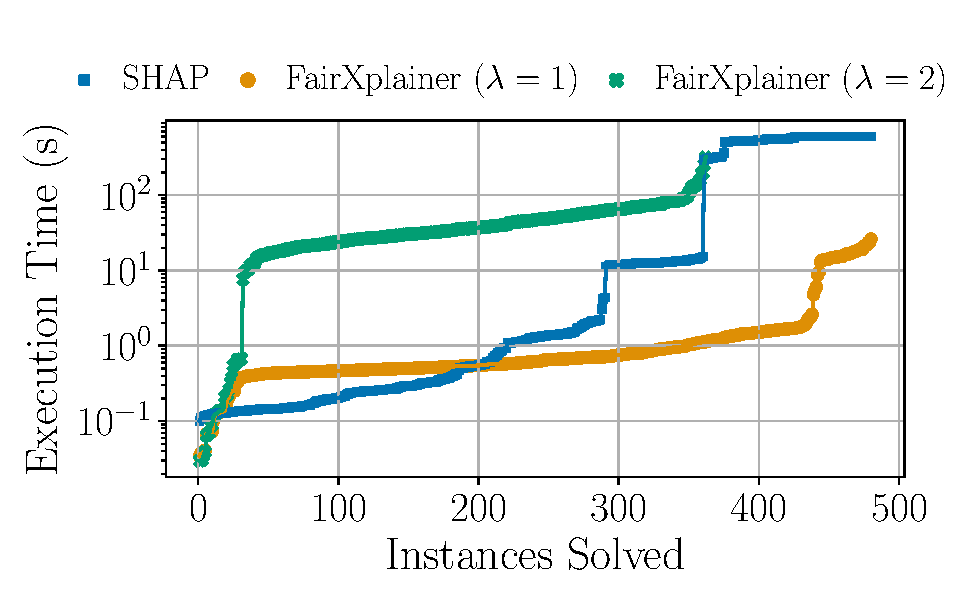
\includegraphics[scale=0.45]{figures/fairness/fif/runtime_diff_methods_train_eo}} 
	\subfloat[Predictive Parity]{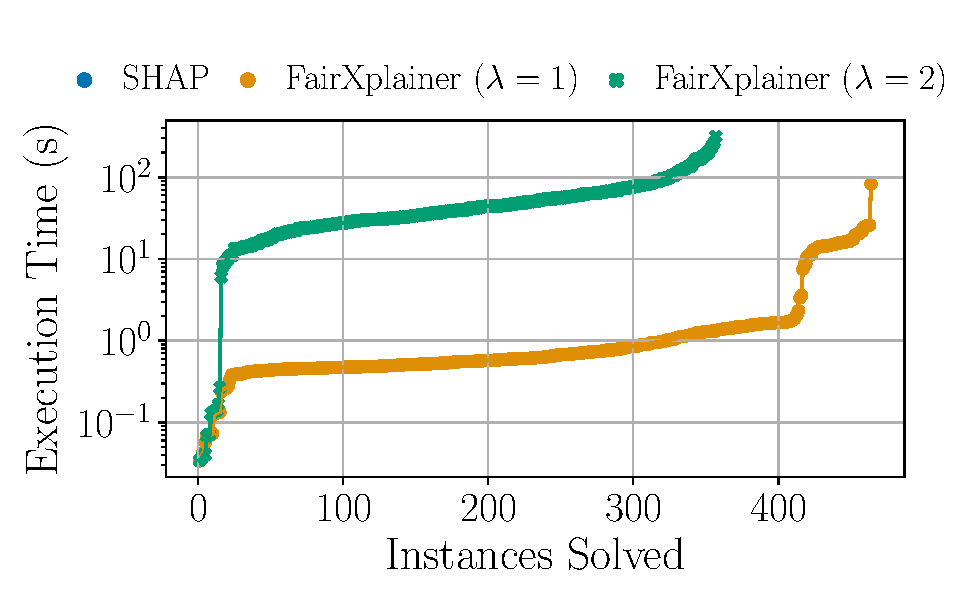
\includegraphics[scale=0.45]{figures/fairness/fif/runtime_diff_methods_train_suff}}
	\caption[Execution time of FIFs]{Execution time of different methods for estimating FIFs for equalized odds and predictive parity. {\fairXplainer} with $ \lambda = 1 $ is more efficient than SHAP, while {\fairXplainer} ($ \lambda = 2 $) requires more computational effort. SHAP cannot explain predictive parity. 
	}
	\label{fairness_fairXplainer_fig:execution_time_cactus_plot_eo_pp}
\end{figure}


\subsection{Execution Time for FIF Estimation of Equalized Odds and Predictive Parity}
In Figure~\ref{fairness_fairXplainer_fig:execution_time_cactus_plot_eo_pp}, we demonstrate the execution time of different methods in estimating FIFs of equalized odds and predictive parity in cactus plots. {\fairXplainer} with $ \lambda = 1 $ is more efficient than $ \lambda = 2 $ and solves all $ 480 $ fairness instances with at least one order of magnitude less execution time. Compared to {\fairXplainer} ($ \lambda = 1 $), SHAP demonstrates less computational efficiency.

\begin{figure}
	\centering
	\subfloat[Adult]{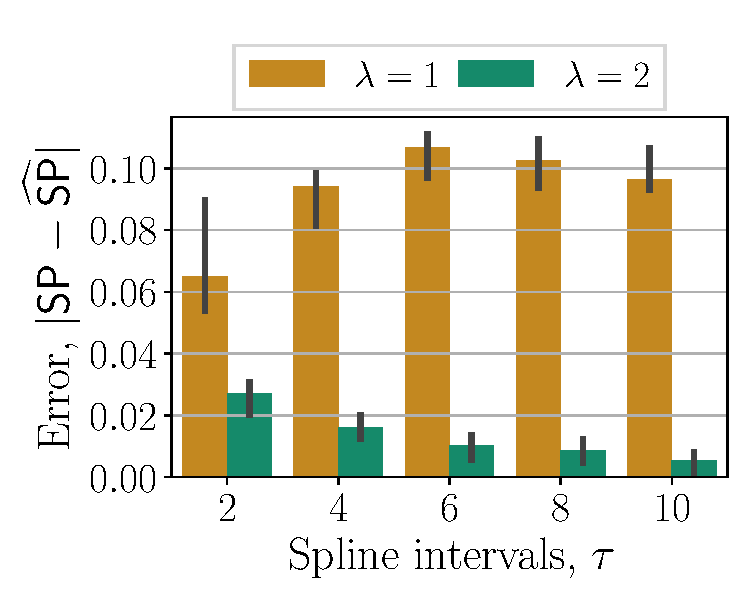
\includegraphics[scale=0.38]{figures/fairness/fif/sp_adult_train_error.pdf}}
	\subfloat[Adult]{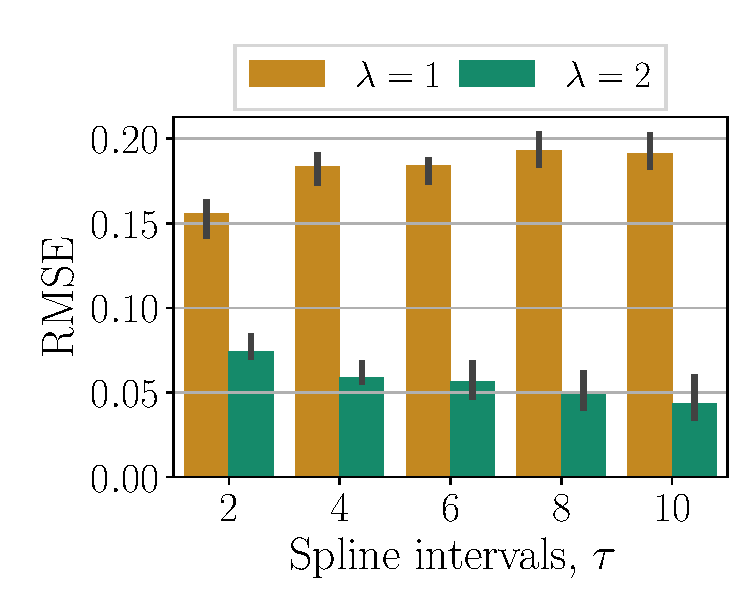
\includegraphics[scale=0.38]{figures/fairness/fif/sp_adult_train_mean_rmse.pdf}}
	\subfloat[Adult]{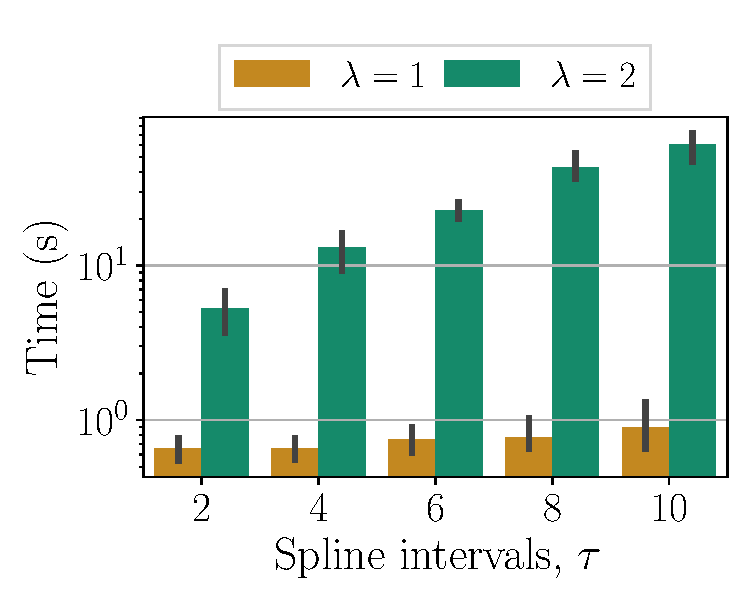
\includegraphics[scale=0.38]{figures/fairness/fif/sp_adult_train_time.pdf}}
	
	\subfloat[COMPAS]{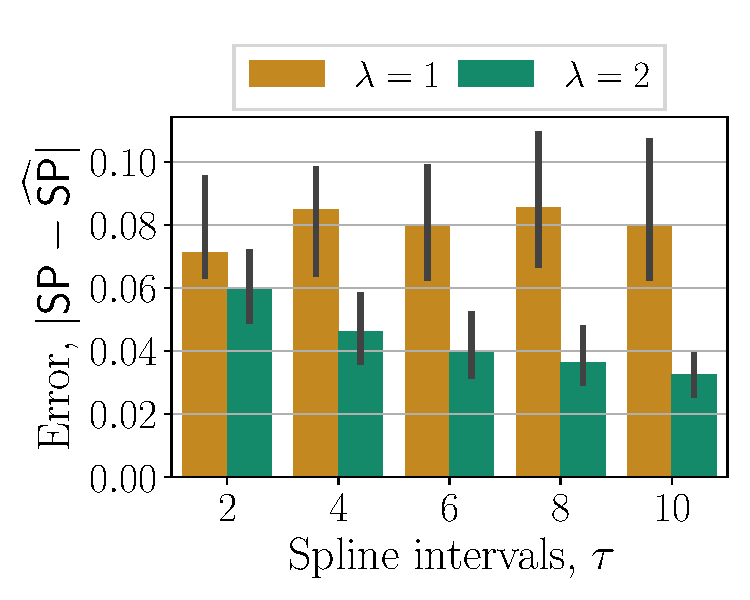
\includegraphics[scale=0.38]{figures/fairness/fif/sp_compas_train_error.pdf}}
	\subfloat[COMPAS]{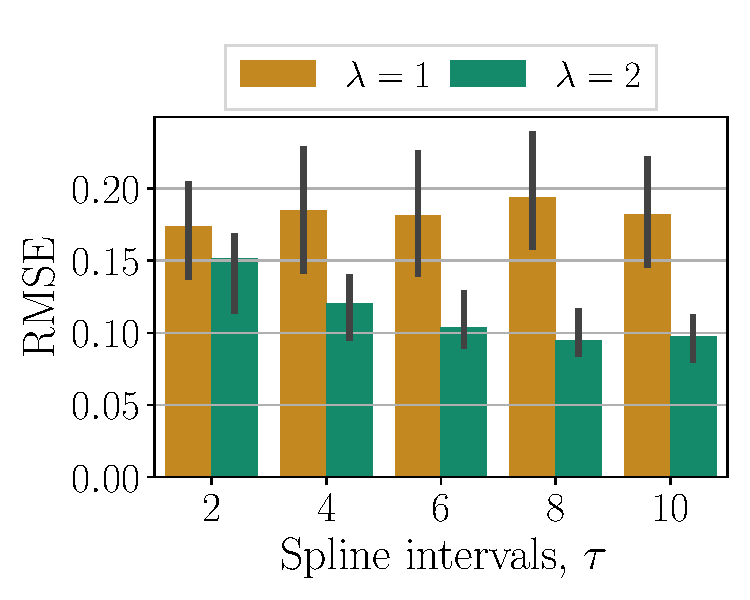
\includegraphics[scale=0.38]{figures/fairness/fif/sp_compas_train_mean_rmse.pdf}}
	\subfloat[COMPAS]{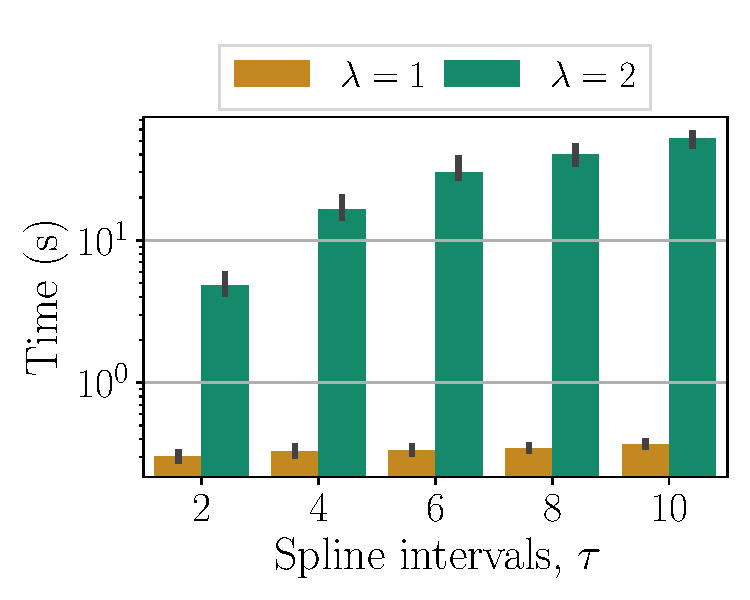
\includegraphics[scale=0.38]{figures/fairness/fif/sp_compas_train_time.pdf}}
	
	\caption[Ablation study on FIFs: effect of spline intervals]{Effect of spline intervals on the approximation error of statistical parity, root-mean square error (RMSE), and  execution time of {\fairXplainer}.}
	\label{fairness_fairXplainer_fig:effect_spline_intervals_appendix}
\end{figure}




\subsection{Ablation Study: Effect of Spline Intervals} 
To understand the impact of spline intervals $\tau$ on {\fairXplainer}, we conduct an experiment. $\tau$ determines the number of local points to include in the cubic-spline based smoothing, with higher values providing better approximation of the component functions in the set-additive decomposition of the classifier (ref.\ Eq.~\eqref{fairness_fairXplainer_eq:set_additive_classifier}). As shown in Figure~\ref{fairness_fairXplainer_fig:effect_spline_intervals_appendix}, as $\tau$ increases, the approximation error of statistical parity based on FIFs decreases as well as the root mean square error of the set-additive approximation of the classifier. On the other hand, with higher $ \tau $, the execution time of {\fairXplainer} increases. Therefore, \emph{$ \tau $ exhibits a trade-off between the estimation accuracy and execution time of {\fairXplainer}.}

\begin{comment}
\subsection{Runtime of {\fairXplainer}} \label{fairness_fairXplainer_sec:runtime_exp}
In Figure~\ref{fairness_fairXplainer_fig:runtime}, we report the runtime of {\fairXplainer} in computing FIFs (with $ \lambda = 2 $) for different group fairness metrics on four classifiers and five datasets. The dimension of the dataset, measured by the number of samples and the number of features, is a key factor for runtime. For example, Adult dataset has the maximum number of samples ($ = 26048 $) compared to other datasets. In contrast, German dataset has the maximum features ($ = 26 $). Consequently, {\fairXplainer} requires more runtime in both Adult and German dataset compared to others. However, \emph{in all datasets, FIF computation takes at most $ 25 $ seconds, that demonstrates the efficiency of {\fairXplainer} in practical fairness problems.}
\end{comment}



\begin{comment}
\begin{figure}
	\centering
	\subfloat[Statistical parity]{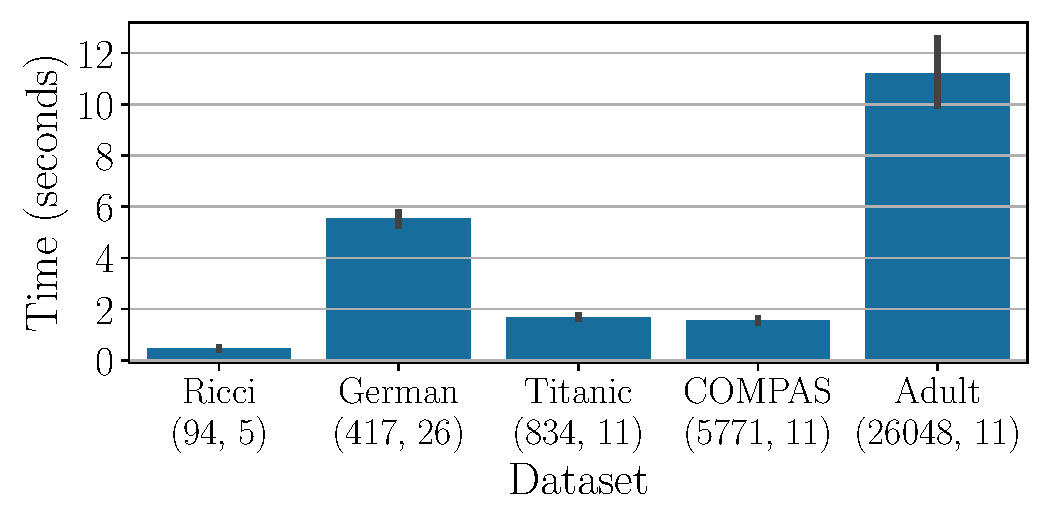
\includegraphics[scale=0.39]{figures/fairness/fif/sp_train_time_detailed_fairXplainer_only}}
	\subfloat[Equalized odds]{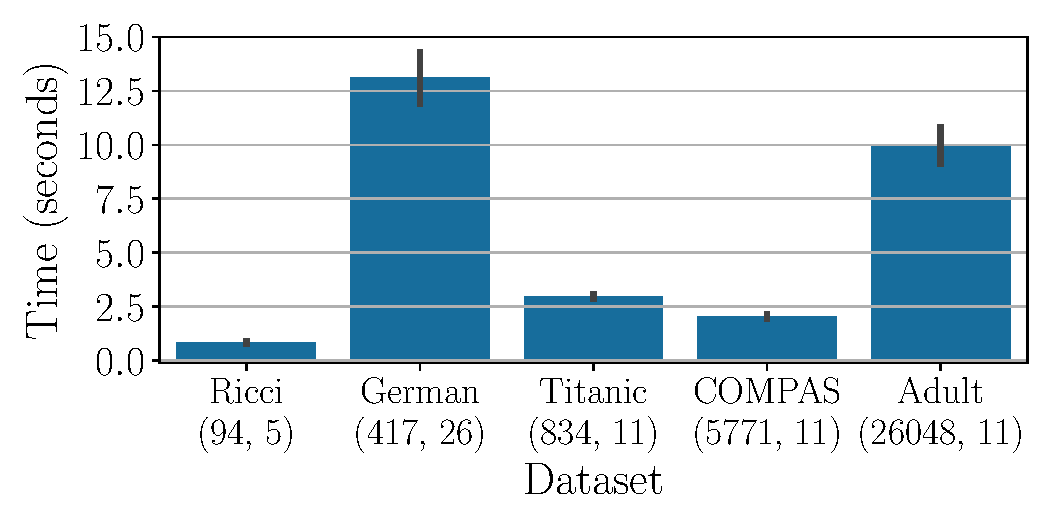
\includegraphics[scale=0.39]{figures/fairness/fif/eo_train_time_detailed_fairXplainer_only}}\\
	\subfloat[Predictive parity]{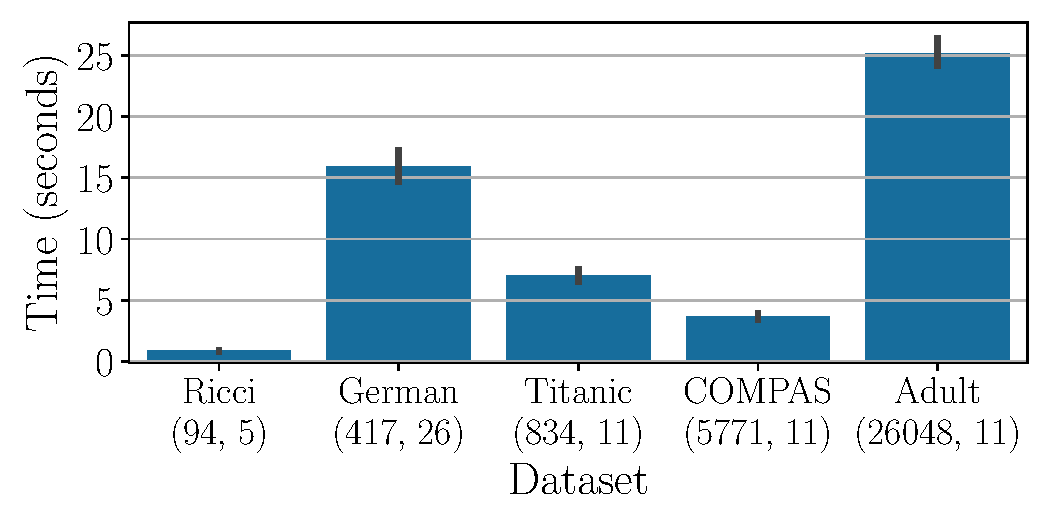
\includegraphics[scale=0.39]{figures/fairness/fif/suff_train_time_detailed_fairXplainer_only}}
	\caption{Runtime of {\fairXplainer} (in seconds) for computing FIFs in different datasets. For each dataset, we mention its dimension as a tuple (\# sample, \# features) in the xticks. As the dimension increases, we observe higher runtime of {\fairXplainer}.}\label{fairness_fairXplainer_fig:runtime}\vspace*{-1em}
\end{figure}
\end{comment}


\begin{figure}
	\centering
	\subfloat{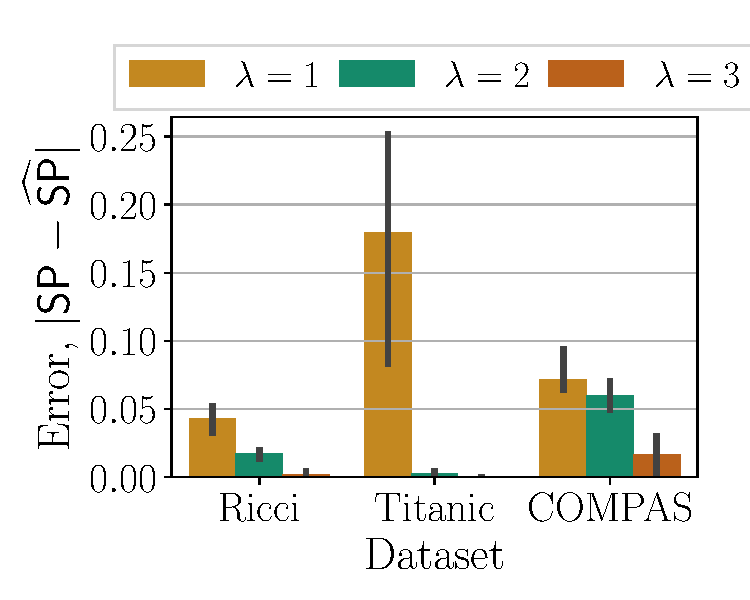
\includegraphics[scale=0.4]{figures/fairness/fif/ablation_study_max_order_sp_train_error.pdf}}
	\subfloat{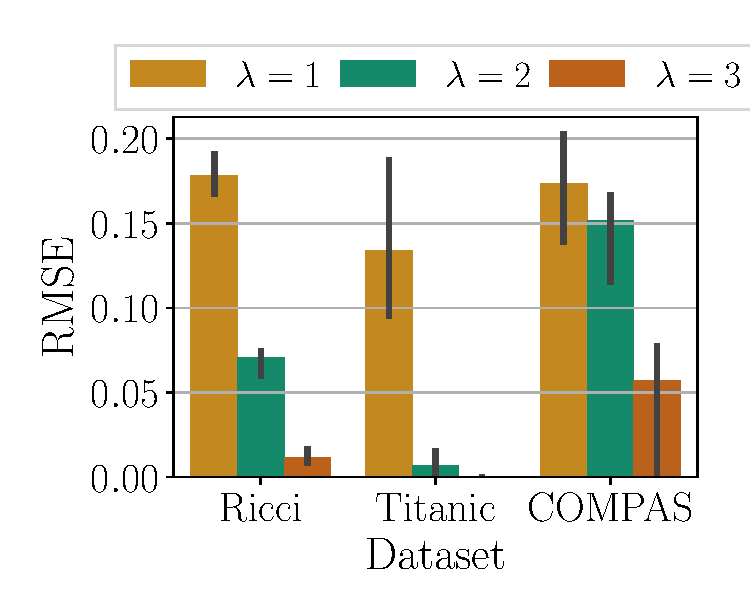
\includegraphics[scale=0.4]{figures/fairness/fif/ablation_study_max_order_sp_train_mean_rmse.pdf}}
	\subfloat{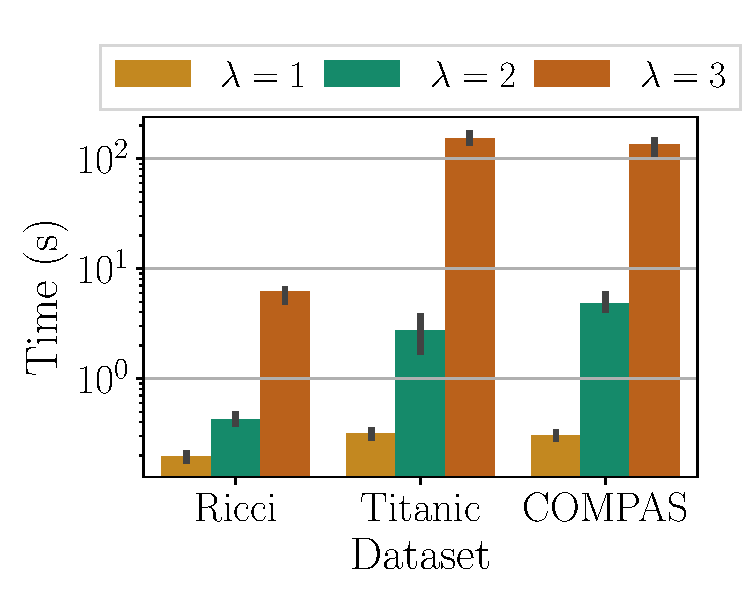
\includegraphics[scale=0.4]{figures/fairness/fif/ablation_study_max_order_sp_train_time.pdf}}
	
	
	\caption[Ablation study on FIFs: effect of maximum order of intersectionality]{Effect of maximum order $ \lambda $ on the approximation error of statistical parity, root-mean square error (RMSE) and  execution time of {\fairXplainer}.}
	\label{fairness_fairXplainer_fig:effect_maxorder_appendix}
\end{figure}




\subsection{Ablation Study: Effect of Maximum Order of Intersectionality}\label{fairness_fairXplainer_sec:ablation} 
Figure~\ref{fairness_fairXplainer_fig:effect_maxorder_appendix} examines the impact of the maximum order of intersectionality ($\lambda$) on {\fairXplainer} in terms of accuracy and execution time on Ricci~\cite{mcginley2010ricci}, Titanic, and COMPAS datasets. As $\lambda$ increases, we see a decrease in approximation error for statistical parity based on FIFs, a decrease in the root mean squared error of the classifier's set additive decomposition, and an increase in execution time across different datasets. This means $\lambda$ provides a trade-off between accuracy and efficiency in {\fairXplainer}.

\begin{comment}
\begin{figure}[t!]
	\centering
	{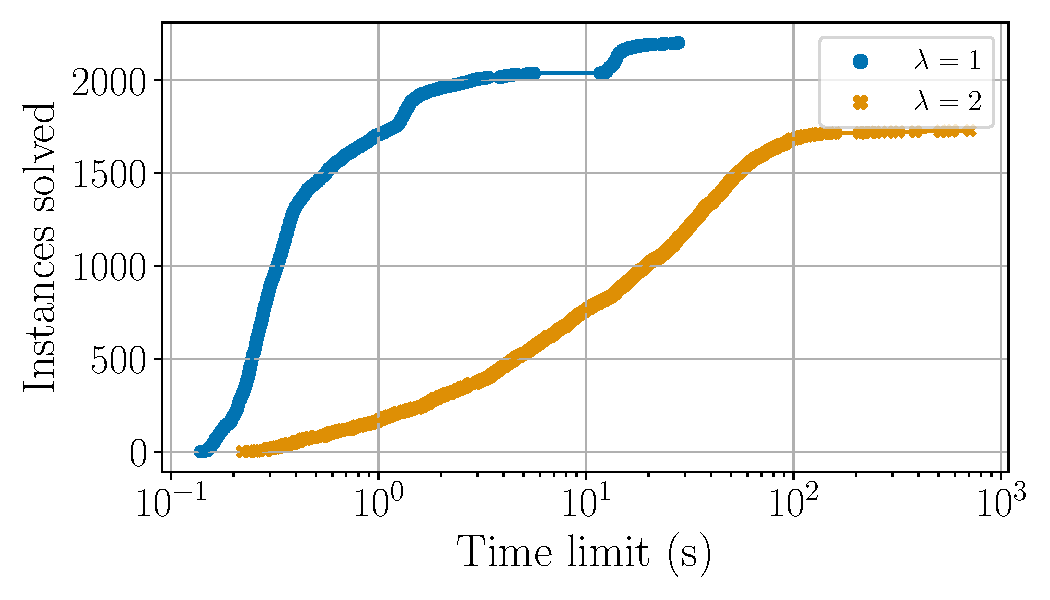
\includegraphics[scale=0.38]{figures/fairness/fif/vary_max_order_train}}
	%	\subfloat[]{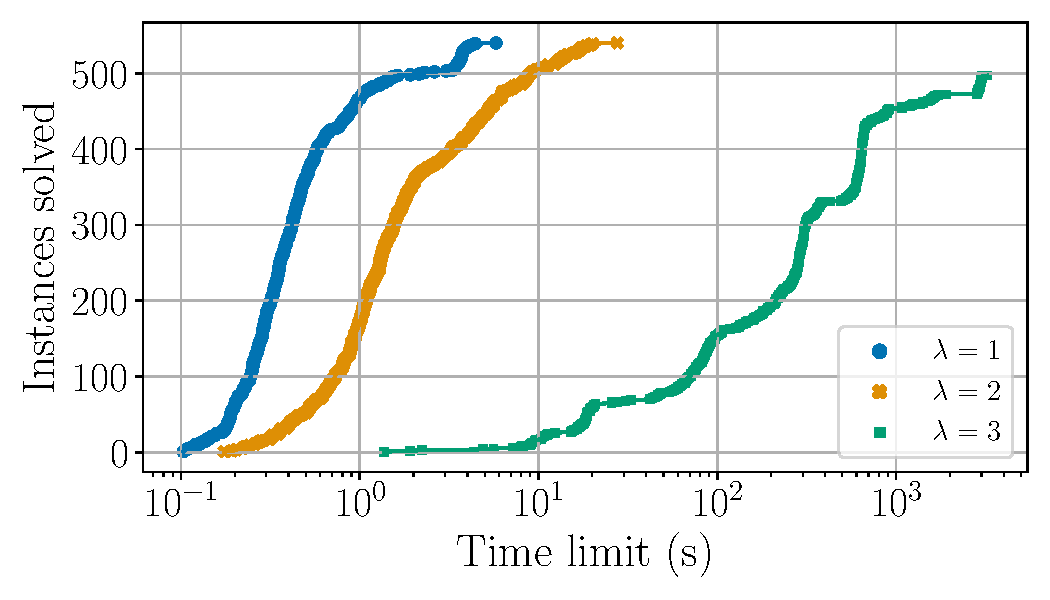
\includegraphics[scale=0.4]{figures/fairness/fif/vary_max_order_test}}	
	\vspace{-1em}
	\caption{Effect on runtime while varying max-order $ \lambda $ in {\fairXplainer}. Higher $ \lambda $ incurs more a computational effort, hereby solving less fairness instances within the same time limit.}\label{fairness_fairXplainer_fig:varying_max_order}
\end{figure}
\end{comment}


\begin{comment}

\begin{table*}    
	\caption{Median estimation error of equalized odds, $ |\mathsf{EO} - \widehat{\mathsf{EO}}| $, in terms of estimated FIFs by different methods (columns $ 5 $ to $ 7 $, less is better). Best results are in bold color. {\textemdash} denotes timeout in estimating FIFs.}
%	\label{fairness_fairXplainer_tab:fair_algo_verification}   
	\centering
	%        \setlength{\tabcolsep}{.3em}
	\begin{tabular}{lrclrrrr}
		\toprule
		\multirow{2}{*}{Dataset} & \multirow{2}{*}{\shortstack[1]{Dimension\\$ (n, \numfeatures) $}} & \multirow{2}{*}{\shortstack[1]{Maximum\\Sensitive Features}} &\multirow{2}{*}{Classifier} & \multirow{2}{*}{SHAP} & \multicolumn{2}{c}{\fairXplainer}\\
		& & & & & $ \lambda = 1 $ & $ \lambda = 2 $\\
		\midrule
		
		
		\multirow{4}{*}{Ricci} & \multirow{4}{*}{$ (94, 5) $} & \multirow{4}{*}{$ 2$} 
		& Logistic Regression &  $ 0.568 $ &  $ 0.002 $ &  $ \mathbf{0.001} $ &  \\ 
		& & & SVM &  $ 0.388 $ &  $ 0.003 $ &  $ \mathbf{0.001} $ &  \\ 
		& & & Neural Network &  $ \mathbf{0.0} $ &  $ 1.0 $ &  $ 1.0 $ &  \\ 
		& & & Decision Tree &  $ \mathbf{0.0} $ &  $ 1.0 $ &  $ 1.0 $ &  \\ 
		\midrule
		
		\multirow{4}{*}{Titanic} & \multirow{4}{*}{$ (834, 11) $} & \multirow{4}{*}{$ 3$} 
		& Logistic Regression &  $ 1.697 $ &  $ \mathbf{0.0} $ &  $ \mathbf{0.0} $ &  \\ 
		& & & SVM &  $ 1.0 $ &  $ \mathbf{0.0} $ &  $ \mathbf{0.0} $ &  \\ 
		& & & Neural Network & \textemdash &  $ \mathbf{0.0} $ &  $ \mathbf{0.0} $ &  \\ 
		& & & Decision Tree &  $ 0.074 $ &  $ 0.185 $ &  $ \mathbf{0.059} $ &  \\ 
		\midrule
		
		\multirow{4}{*}{German} & \multirow{4}{*}{$ (417, 23) $} & \multirow{4}{*}{$ 2$} 
		& Logistic Regression &  $ 0.382 $ &  $ 0.109 $ &  $ \mathbf{0.001} $ &  \\ 
		& & & SVM &  $ 0.435 $ &  $ \mathbf{0.082} $ & \textemdash &  \\ 
		& & & Neural Network & \textemdash &  $ 0.149 $ &  $ \mathbf{0.0} $ &  \\ 
		& & & Decision Tree &  $ \mathbf{0.0} $ &  $ 1.0 $ &  $ 1.0 $ &  \\ 
		\midrule
		
		\multirow{4}{*}{COMPAS} & \multirow{4}{*}{$ (5771, 8) $} & \multirow{4}{*}{$ 3$} 
		& Logistic Regression &  $ 0.38 $ &  $ 0.167 $ &  $ \mathbf{0.071} $ &  \\ 
		& & & SVM &  $ 0.481 $ &  $ 0.043 $ &  $ \mathbf{0.024} $ &  \\ 
		& & & Neural Network & \textemdash &  $ 0.143 $ &  $ \mathbf{0.055} $ &  \\ 
		& & & Decision Tree &  $ 0.071 $ &  $ 0.069 $ &  $ \mathbf{0.031} $ &  \\ 
		\midrule
		
		\multirow{4}{*}{Adult} & \multirow{4}{*}{$ (26048, 11) $} & \multirow{4}{*}{$ 3$} 
		& Logistic Regression &  $ 1.647 $ &  $ 0.186 $ &  $ \mathbf{0.013} $ &  \\ 
		& & & SVM &  $ 0.703 $ &  $ 0.081 $ &  $ \mathbf{0.001} $ &  \\ 
		& & & Neural Network & \textemdash &  $ 0.077 $ &  $ \mathbf{0.0} $ &  \\ 
		& & & Decision Tree &  $ \mathbf{0.062} $ &  $ 0.263 $ &  $ 0.2 $ &  \\ 
		
		
		\bottomrule
	\end{tabular}
\end{table*}

\begin{table*}    
	\caption{Median estimation error of predictive parity, $ |\mathsf{PP} - \widehat{\mathsf{PP}}| $, in terms of estimated FIFs by different methods (columns $ 5 $ to $ 7 $, less is better). Best results are in bold color. {\textemdash} denotes timeout in estimating FIFs.}
	%	\label{fairness_fairXplainer_tab:fair_algo_verification}   
	\centering
	%        \setlength{\tabcolsep}{.3em}
	\begin{tabular}{lrclrrrr}
		\toprule
		\multirow{2}{*}{Dataset} & \multirow{2}{*}{\shortstack[1]{Dimension\\$ (n, \numfeatures) $}} & \multirow{2}{*}{\shortstack[1]{Maximum\\Sensitive Features}} &\multirow{2}{*}{Classifier} & \multirow{2}{*}{SHAP} & \multicolumn{2}{c}{\fairXplainer}\\
		& & & & & $ \lambda = 1 $ & $ \lambda = 2 $\\
		\midrule
		
		
		\multirow{4}{*}{Ricci} & \multirow{4}{*}{$ (94, 5) $} & \multirow{4}{*}{$ 2$} 
		& Logistic Regression & \textemdash &  $ 0.006 $ &  $ \mathbf{0.001} $ &  \\ 
		& & & SVM & \textemdash &  $ 0.018 $ &  $ \mathbf{0.0} $ &  \\ 
		& & & Neural Network & \textemdash &  $ \mathbf{1.0} $ &  $ \mathbf{1.0} $ &  \\ 
		& & & Decision Tree & \textemdash &  $ \mathbf{1.0} $ &  $ \mathbf{1.0} $ &  \\ 
		\midrule
		
		\multirow{4}{*}{Titanic} & \multirow{4}{*}{$ (834, 11) $} & \multirow{4}{*}{$ 3$} 
		& Logistic Regression & \textemdash &  $ 0.251 $ &  $ \mathbf{0.148} $ &  \\ 
		& & & SVM & \textemdash &  $ 0.092 $ &  $ \mathbf{0.049} $ &  \\ 
		& & & Neural Network & \textemdash &  $ 0.349 $ &  $ \mathbf{0.171} $ &  \\ 
		& & & Decision Tree & \textemdash &  $ \mathbf{0.097} $ &  $ \mathbf{0.097} $ &  \\ 
		\midrule
		
		\multirow{4}{*}{German} & \multirow{4}{*}{$ (417, 23) $} & \multirow{4}{*}{$ 2$} 
		& Logistic Regression & \textemdash &  $ 0.075 $ &  $ \mathbf{0.001} $ &  \\ 
		& & & SVM & \textemdash &  $ 0.06 $ &  $ \mathbf{0.001} $ &  \\ 
		& & & Neural Network & \textemdash &  $ 0.184 $ &  $ \mathbf{0.0} $ &  \\ 
		& & & Decision Tree & \textemdash &  $ \mathbf{1.0} $ &  $ \mathbf{1.0} $ &  \\ 
		\midrule
		
		\multirow{4}{*}{COMPAS} & \multirow{4}{*}{$ (5771, 8) $} & \multirow{4}{*}{$ 3$} 
		& Logistic Regression & \textemdash &  $ \mathbf{0.201} $ &  $ 0.214 $ &  \\ 
		& & & SVM & \textemdash &  $ 0.124 $ &  $ \mathbf{0.117} $ &  \\ 
		& & & Neural Network & \textemdash &  $ \mathbf{0.078} $ &  $ 0.129 $ &  \\ 
		& & & Decision Tree & \textemdash &  $ 0.348 $ &  $ \mathbf{0.34} $ &  \\ 
		\midrule
		
		\multirow{4}{*}{Adult} & \multirow{4}{*}{$ (26048, 11) $} & \multirow{4}{*}{$ 3$} 
		& Logistic Regression & \textemdash &  $ 0.09 $ &  $ \mathbf{0.002} $ &  \\ 
		& & & SVM & \textemdash &  $ 0.109 $ &  $ \mathbf{0.002} $ &  \\ 
		& & & Neural Network & \textemdash &  $ 0.091 $ &  $ \mathbf{0.002} $ &  \\ 
		& & & Decision Tree & \textemdash &  $ 0.216 $ &  $ \mathbf{0.154} $ &  \\ 
		
		
		\bottomrule
	\end{tabular}
\end{table*}


\end{comment}


\begin{comment}
\subsection{Accuracy in Estimating Different Fairness Metrics}
We compare and evaluate the accuracies of {\fairXplainer} and SHAP in estimating a fairness metric, computed as the sum of FIFs. We illustrate the results with a scatter-plot in Figure~\ref{fairness_fairXplainer_fig:accuracy_scatter_plot}. In the plot, each dot represents the estimation of a fairness metric on a dataset and a classifier. 

The majority of dots for {\fairXplainer} are on the line connecting $ (0, 0) $ to $ (1, 1) $  in Figure~\ref{fairness_fairXplainer_fig:accuracy_scatter_plot}. This implies that the estimation of {\fairXplainer} is significantly accurate. Interestingly, error rarely occurs in {\fairXplainer} due to the degenerate cases mentioned in Section~\ref{fairness_fairXplainer_sec:fifs}. 
In contrast, SHAP often computes a metric inaccurately, thereby showing the drawback of applying a local explanation approach for FIF computation. \emph{Thus, {\fairXplainer} is significantly more accurate than SHAP in computing FIFs and the corresponding fairness metrics.}


\begin{figure}[t!]\vspace*{-1em}
	\centering
	\subfloat[Statistical parity]{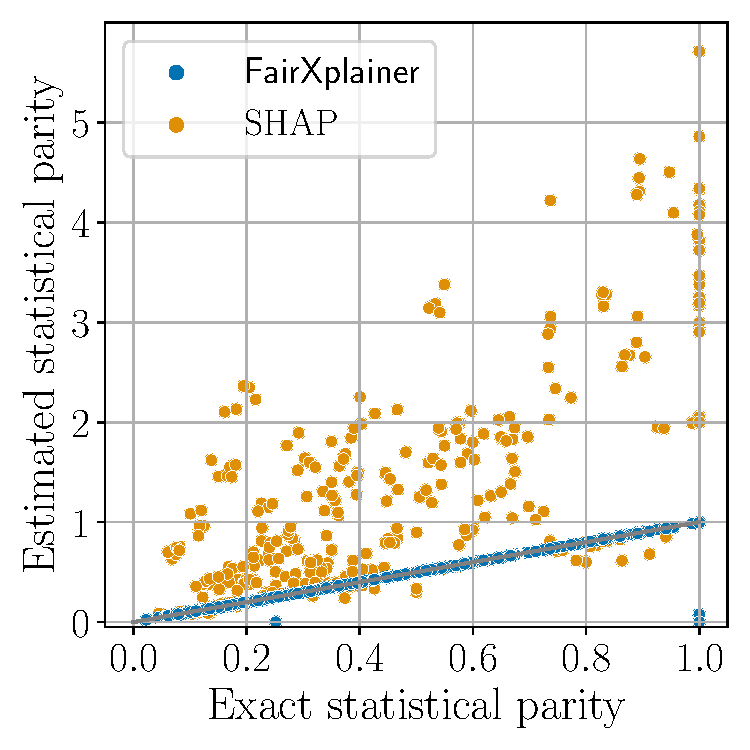
\includegraphics[scale=0.35]{figures/fairness/fif/scatter_plot_sp_train_accuracy}}
	\subfloat[Equalized odds]{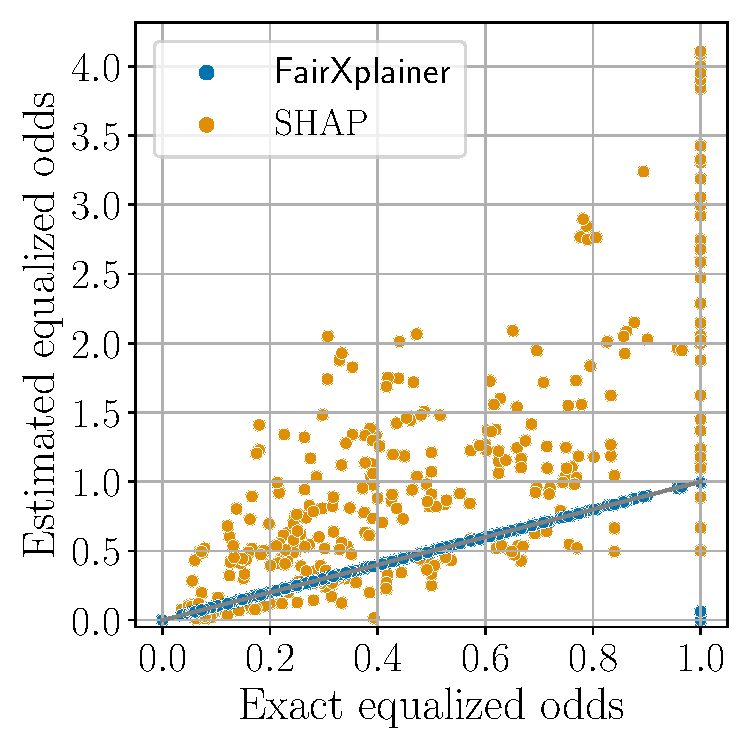
\includegraphics[scale=0.35]{figures/fairness/fif/scatter_plot_eo_train_accuracy}}
	\subfloat[Predictive parity]{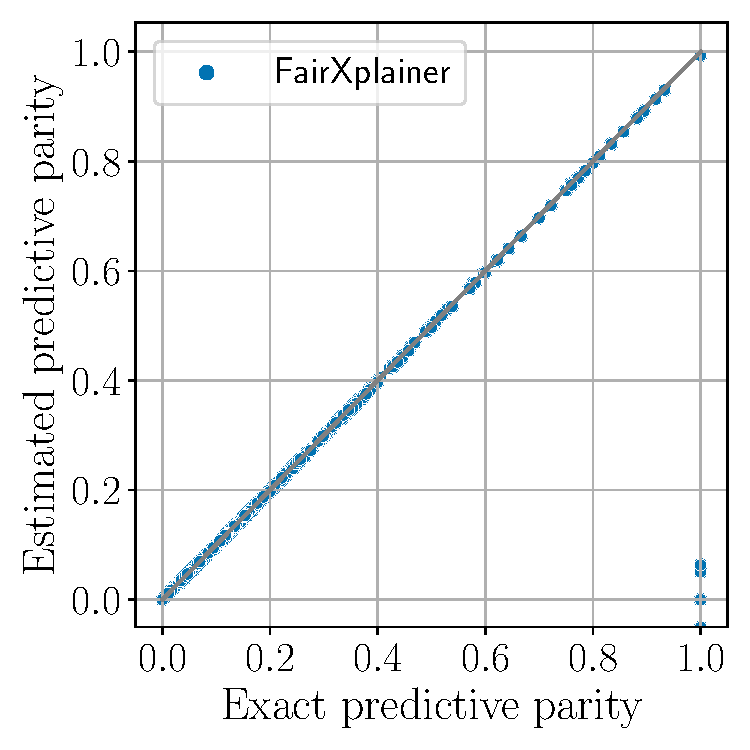
\includegraphics[scale=0.35]{figures/fairness/fif/scatter_plot_suff_train_accuracy}}
	\caption{Comparison between the estimated and exact value of a fairness metric, computed as the sum of FIFs according to Axiom~\ref{fairness_fairXplainer_axm:additivity}. Results are presented separately for {\fairXplainer} and SHAP. Each dot represents the result for a fairness metric, carried over multiple datasets and classifiers. Ideally, if a dot lies on the line connecting $ (0,0) $ to $ (1,1) $, it denotes a correct fairness estimate. {\fairXplainer} demonstrates significantly better accuracy of estimation than SHAP. For predictive parity metric, only {\fairXplainer} allows associated FIFs computation.}
	\label{fairness_fairXplainer_fig:accuracy_scatter_plot}
\end{figure}


\end{comment}



\subsection{FIF of Different Datasets}
We deploy a neural network ($ 3 $ hidden layers, each with $ 2 $ neurons, L$ 2 $ penalty regularization term as $ 10^{-5} $, a constant learning rate as $ 0.001 $) on different datasets, namely Adult and Titanic, and demonstrate the corresponding FIFs in Figures~\ref{fairness_fairXplainer_fig:individual_vs_intersectional_influence_adult} and \ref{fairness_fairXplainer_fig:individual_vs_intersectional_influence_titanic}, respectively. In all the figures, both individual and intersectional FIFs depict the sources of bias more clearly than individual FIFs alone, as argued in Section~\ref{fairness_fairXplainer_sec:experiments}. 


\textbf{In Adult dataset,} the classifier predicts whether an individual earns more than $ \$50 $k per year or not, where race and sex are sensitive features. We observe that the trained network is unfair and it demonstrates statistical parity as $ 0.23 $. As we analyze FIFs,  education number, age, and capital gain/loss are key features responsible for the bias. 

\begin{figure}
	\begin{minipage}{0.45\textwidth}
		\centering
		\subfloat[Individual FIFs]{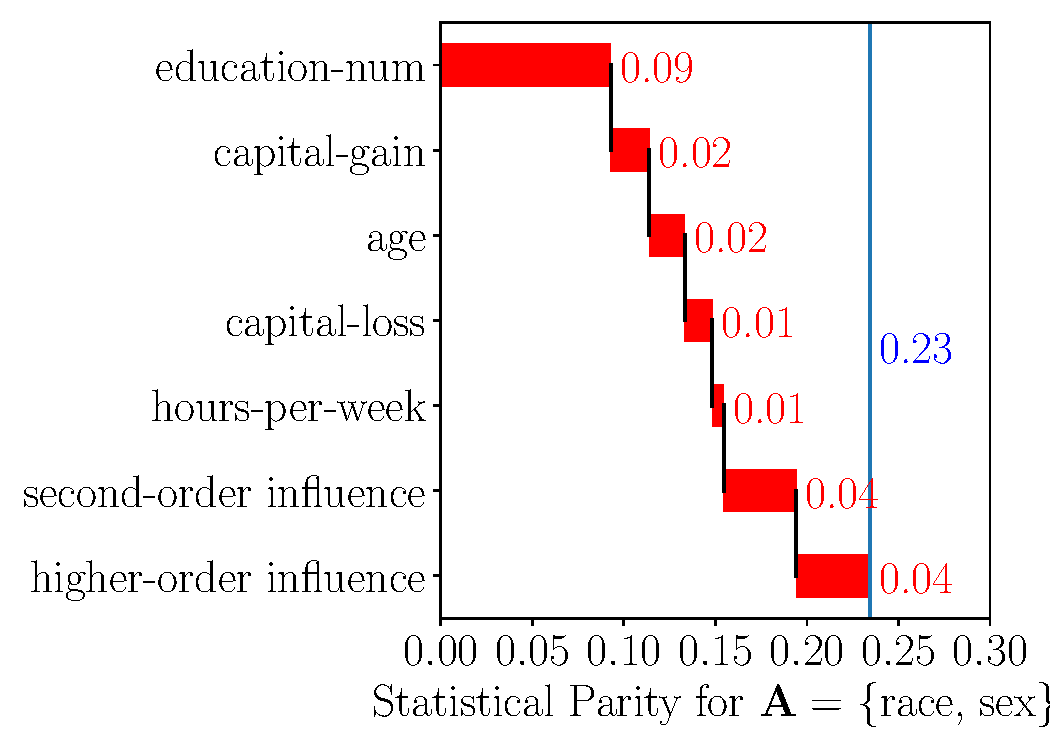
\includegraphics[scale=0.45]{figures/fairness/fif/adult_feature_weight_unsorted}\label{fairness_fairXplainer_fig:individual_fifs_adult}}
	\end{minipage}
	\begin{minipage}{0.5\textwidth}
		\centering
		\subfloat[Individual and intersectional FIFs]{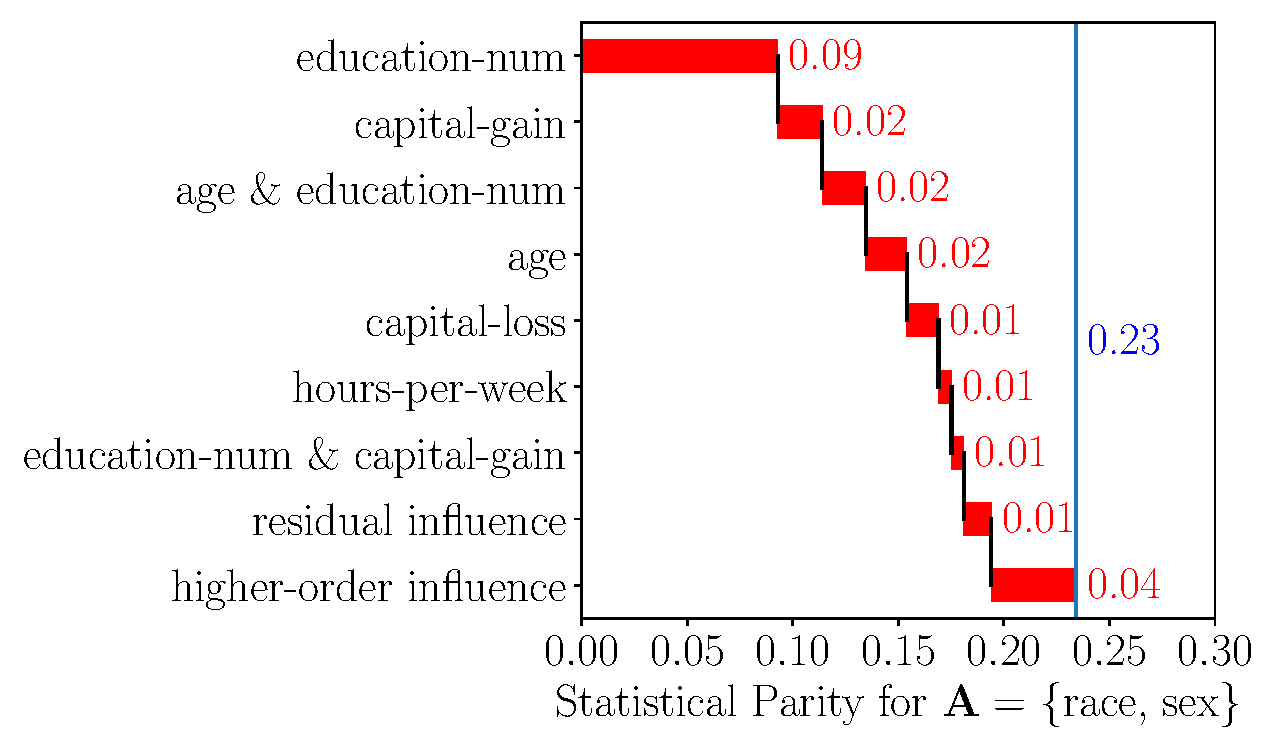
\includegraphics[scale=0.45]{figures/fairness/fif/adult_feature_weight}\label{fairness_fairXplainer_fig:individual_and_intersectional_fifs_adult}}
	\end{minipage}
	\caption[FIFs for Adult dataset]{FIFs for Adult dataset on explaining statistical parity.}\label{fairness_fairXplainer_fig:individual_vs_intersectional_influence_adult}
\end{figure}


\begin{comment}
\textbf{In Ricci dataset,} the classification task  is to predict whether a firefighter obtains promotion or not in New Haven, Connecticut administered exams. We consider `race' as the sensitive feature for this experiment. We observed that the classifier has statistical parity of $ 0.3 $ based on the race of a person. In the computed FIFs, the \textit{combined score} and \textit{desired position} of a person increases bias, whereas written exam score reduces bias while interacting with other features. In addition, the higher order influences demonstrate a higher value (FIF $ = 0.26 $), meaning that the features are highly correlated and act in favor of bias.
\begin{figure}
	\begin{minipage}{0.45\textwidth}
		\centering
		\subfloat[Individual FIFs]{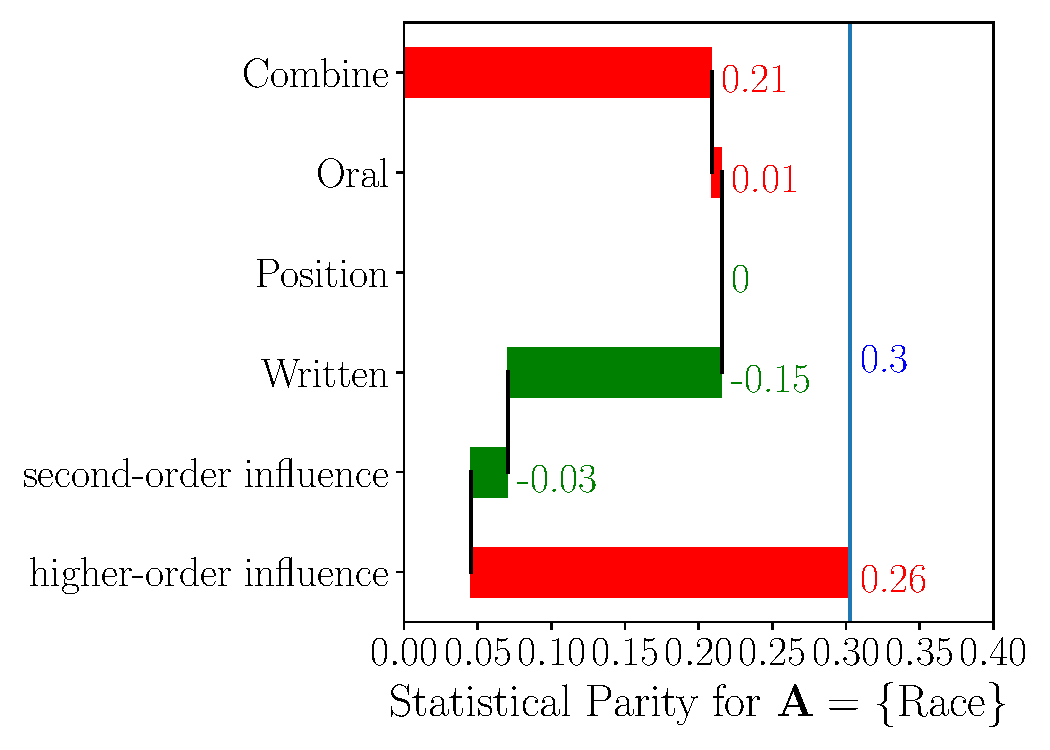
\includegraphics[scale=0.35]{figures/fairness/fif/ricci_feature_weight_unsorted}\label{fairness_fairXplainer_fig:individual_fifs_ricci}}
	\end{minipage}
	\begin{minipage}{0.5\textwidth}
		\centering
		\subfloat[Individual and intersectional FIFs]{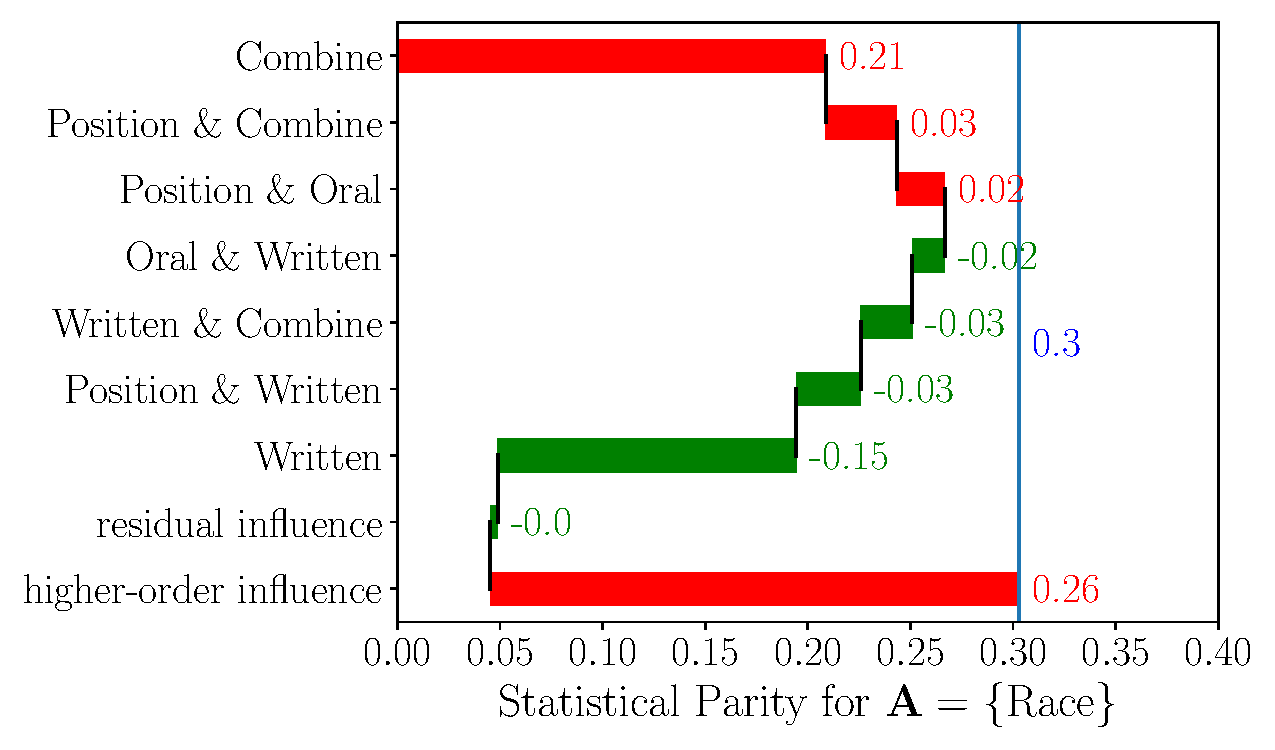
\includegraphics[scale=0.35]{figures/fairness/fif/ricci_feature_weight}\label{fairness_fairXplainer_fig:individual_and_intersectional_fifs_ricci}}
	\end{minipage}
	\vspace{-0.2em}
	\caption{FIFs for Ricci dataset on explaining statistical parity.}\label{fairness_fairXplainer_fig:individual_vs_intersectional_influence_ricci}
\end{figure}

\end{comment}


\textbf{In Titanic dataset,} the neural network predicts whether a person survives the Titanic shipwreck or not. In this experiment, we consider the sex of a person as a sensitive feature and observe that the classifier is highly unfair achieving statistical parity as $ 0.83 $. Our FIF analysis reveals high correlation in Titanic, where individual FIFs are mostly zero while intersectional FIFs achieve high absolute values.

\begin{figure}
	\centering
	\subfloat[Individual FIFs]{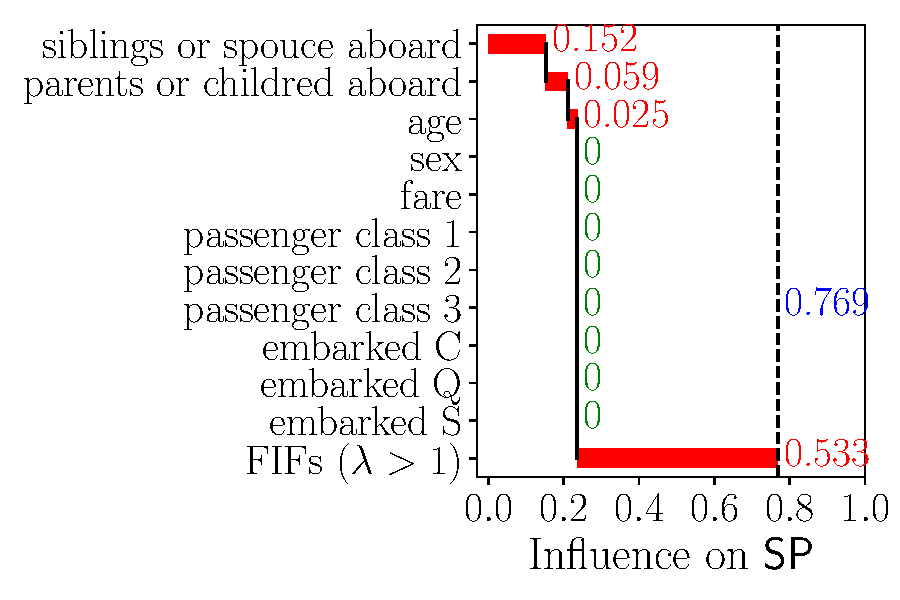
\includegraphics[scale=0.45]{figures/fairness/fif/titanic_feature_weight_unsorted}\label{fairness_fairXplainer_fig:individual_fifs_titanic}}\hfil
	\subfloat[Individual and intersectional FIFs]{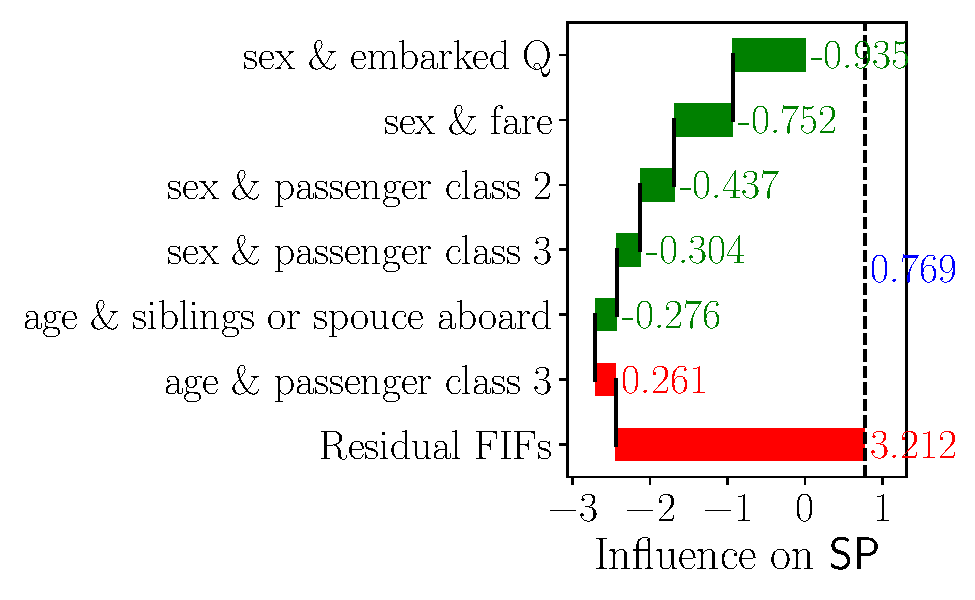
\includegraphics[scale=0.45]{figures/fairness/fif/titanic_feature_weight}\label{fairness_fairXplainer_fig:individual_and_intersectional_fifs_titanic}}
	\caption[FIFs for Titanic dataset]{FIFs for Titanic dataset on explaining statistical parity.}\label{fairness_fairXplainer_fig:individual_vs_intersectional_influence_titanic}
\end{figure}


\begin{comment}

\begin{figure}
	\subfloat{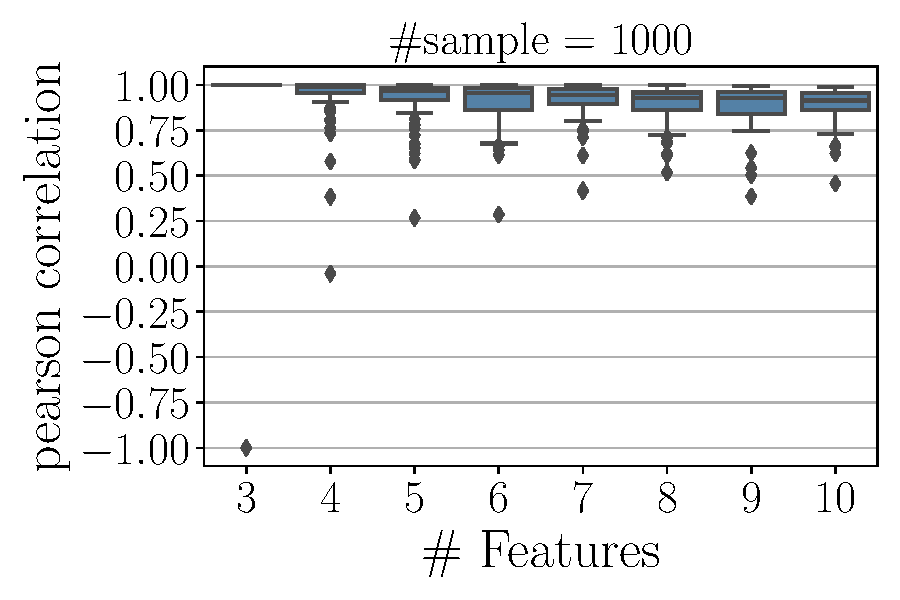
\includegraphics[scale=0.4]{figures/fairness/fif/fairXplainer_sanity_check_1000_0_0_2_0_5_pearson_correlation_.pdf}}
	\subfloat{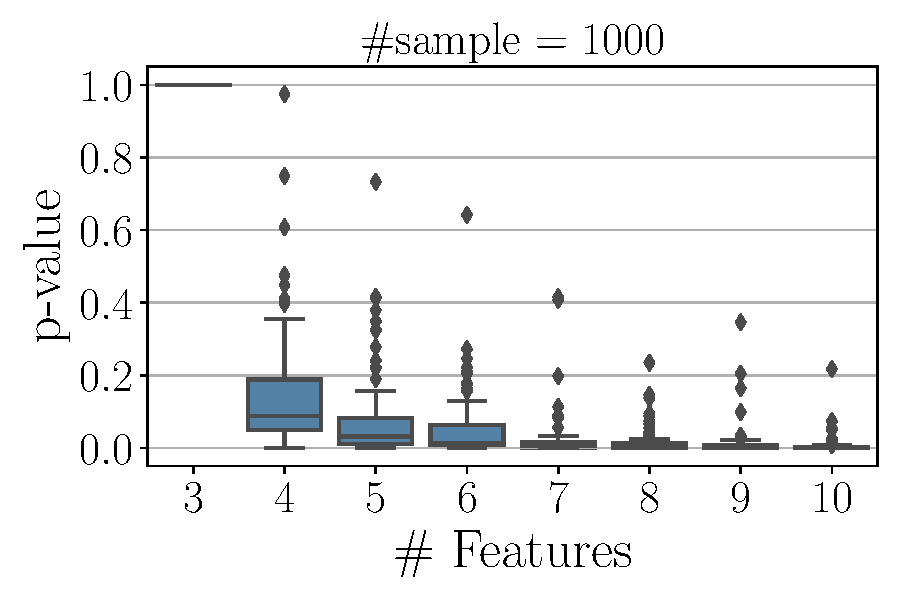
\includegraphics[scale=0.4]{figures/fairness/fif/fairXplainer_sanity_check_1000_0_0_2_0_5_p-value_.pdf}}
	\subfloat{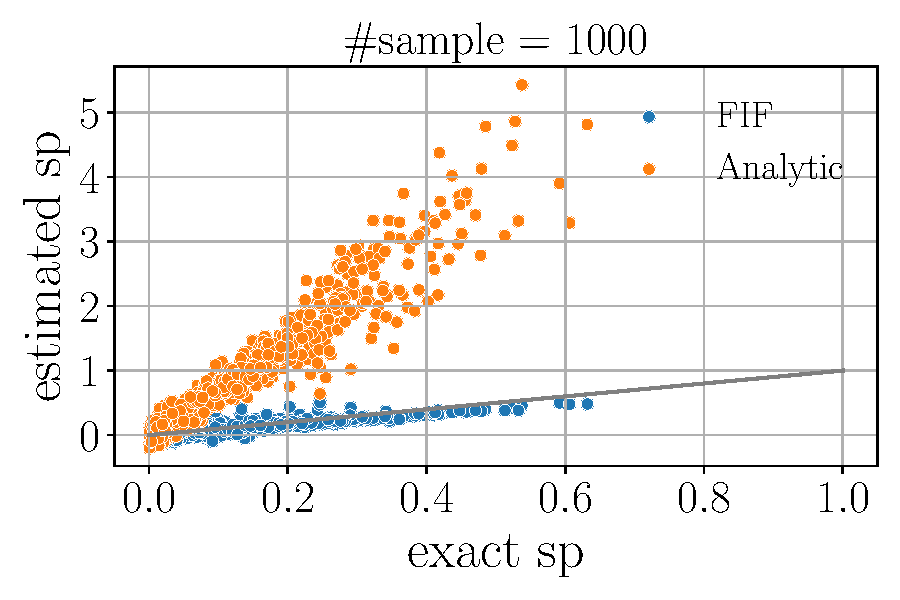
\includegraphics[scale=0.4]{figures/fairness/fif/fairXplainer_sanity_check_1000_0_0_2_0_5_scatter_accuracy_.pdf}}
	
	\subfloat{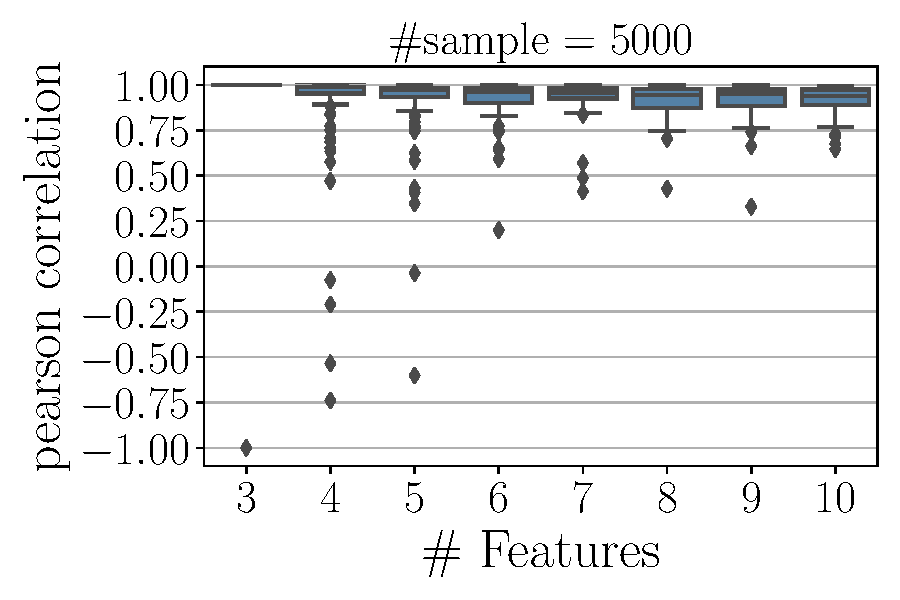
\includegraphics[scale=0.4]{figures/fairness/fif/fairXplainer_sanity_check_5000_0_0_2_0_5_pearson_correlation_.pdf}}
	\subfloat{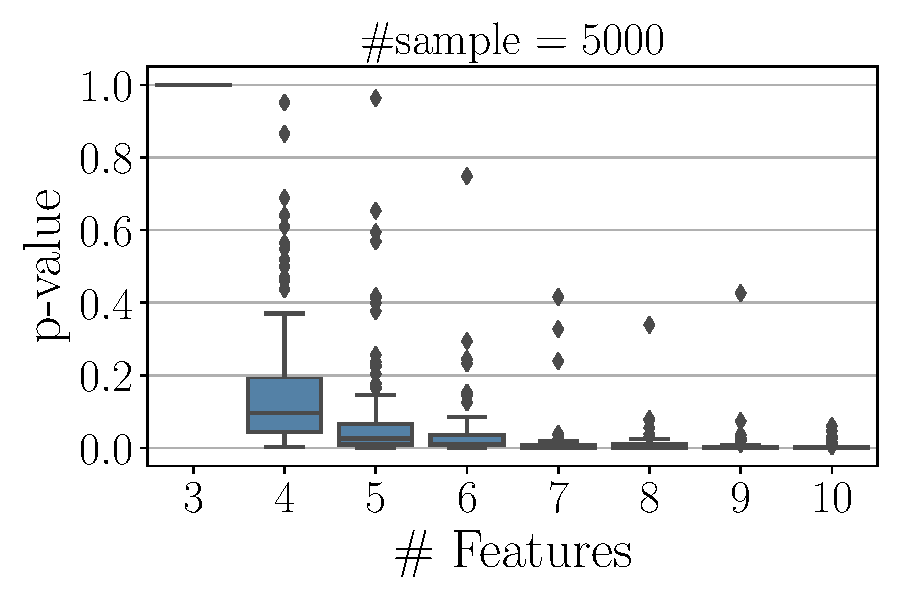
\includegraphics[scale=0.4]{figures/fairness/fif/fairXplainer_sanity_check_5000_0_0_2_0_5_p-value_.pdf}}
	\subfloat{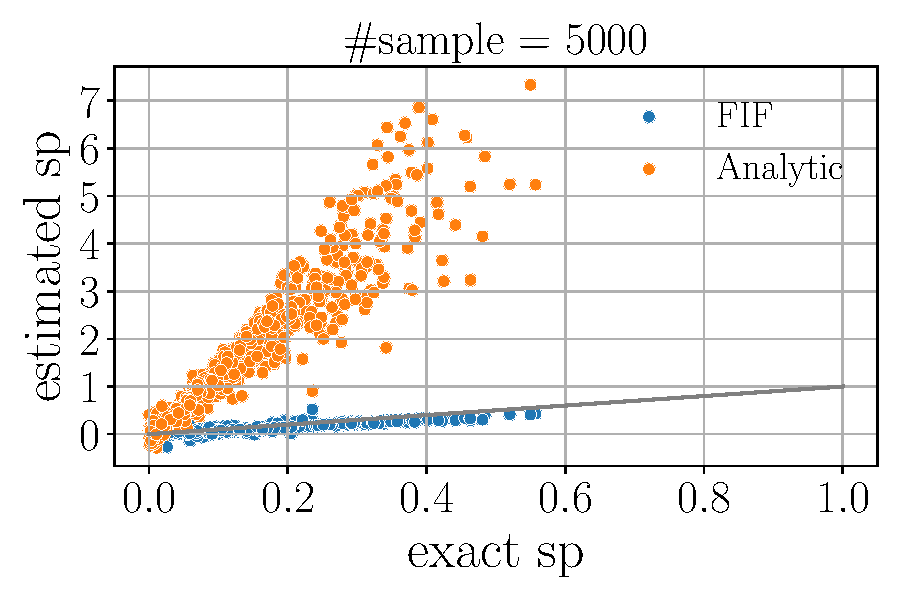
\includegraphics[scale=0.4]{figures/fairness/fif/fairXplainer_sanity_check_5000_0_0_2_0_5_scatter_accuracy_.pdf}}
	
	
	\subfloat{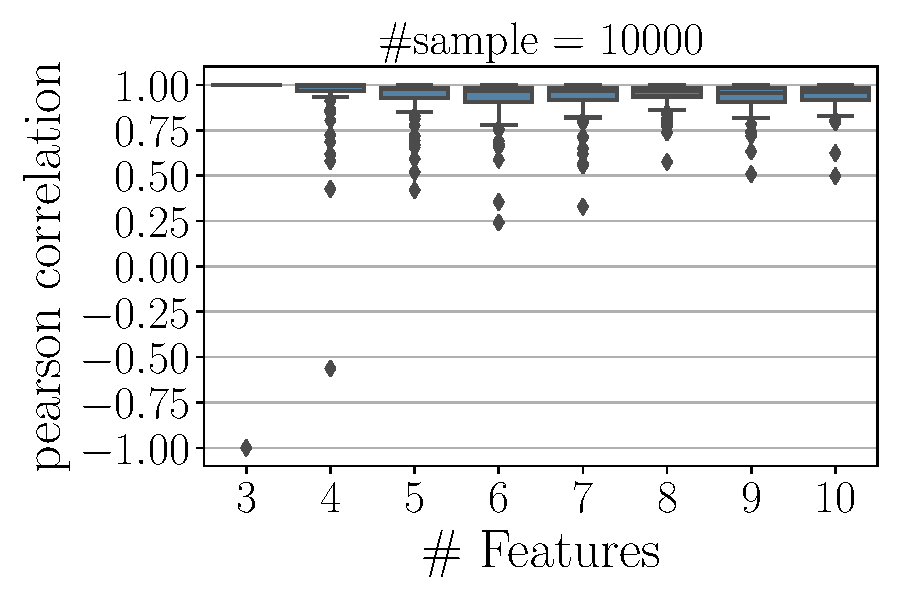
\includegraphics[scale=0.4]{figures/fairness/fif/fairXplainer_sanity_check_10000_0_0_2_0_5_pearson_correlation_.pdf}}
	\subfloat{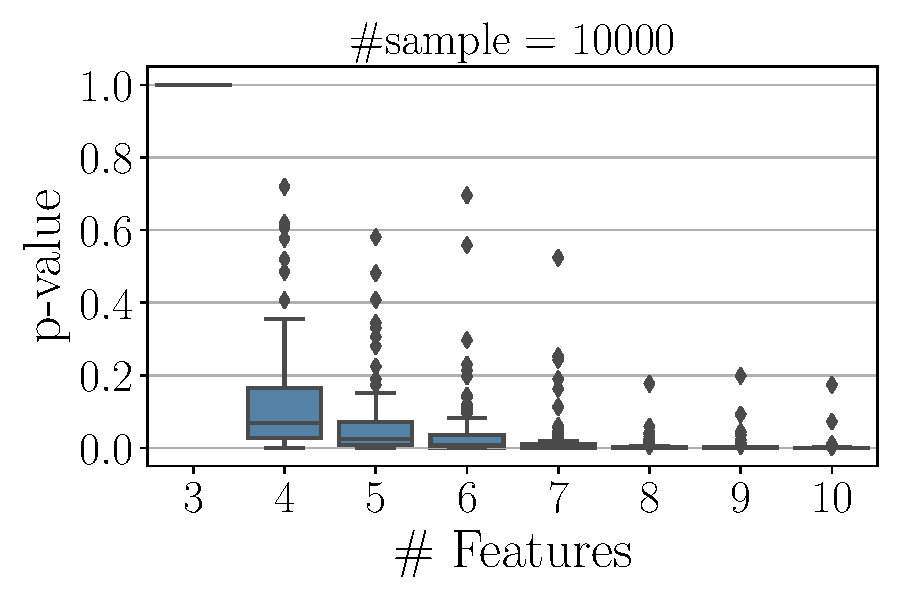
\includegraphics[scale=0.4]{figures/fairness/fif/fairXplainer_sanity_check_10000_0_0_2_0_5_p-value_.pdf}}
	\subfloat{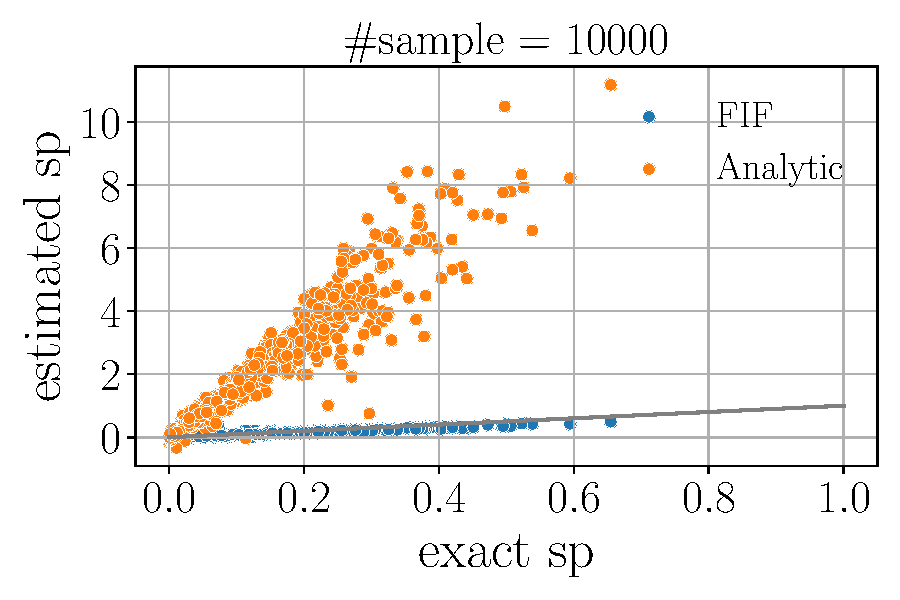
\includegraphics[scale=0.4]{figures/fairness/fif/fairXplainer_sanity_check_10000_0_0_2_0_5_scatter_accuracy_.pdf}}
\end{figure}

\end{comment}



\begin{comment}
\begin{figure}[t!]
	\subfloat[COMPAS]{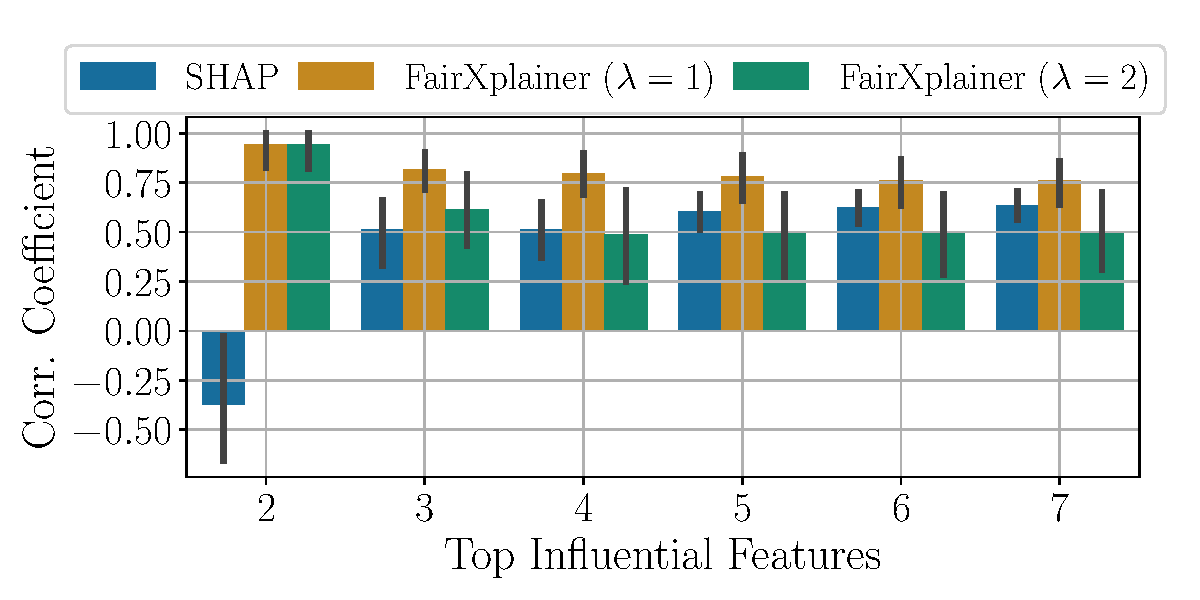
\includegraphics[scale=0.35]{figures/fairness/fif/intervention_compas_intersectional}}\hfil
	\subfloat[Adult]{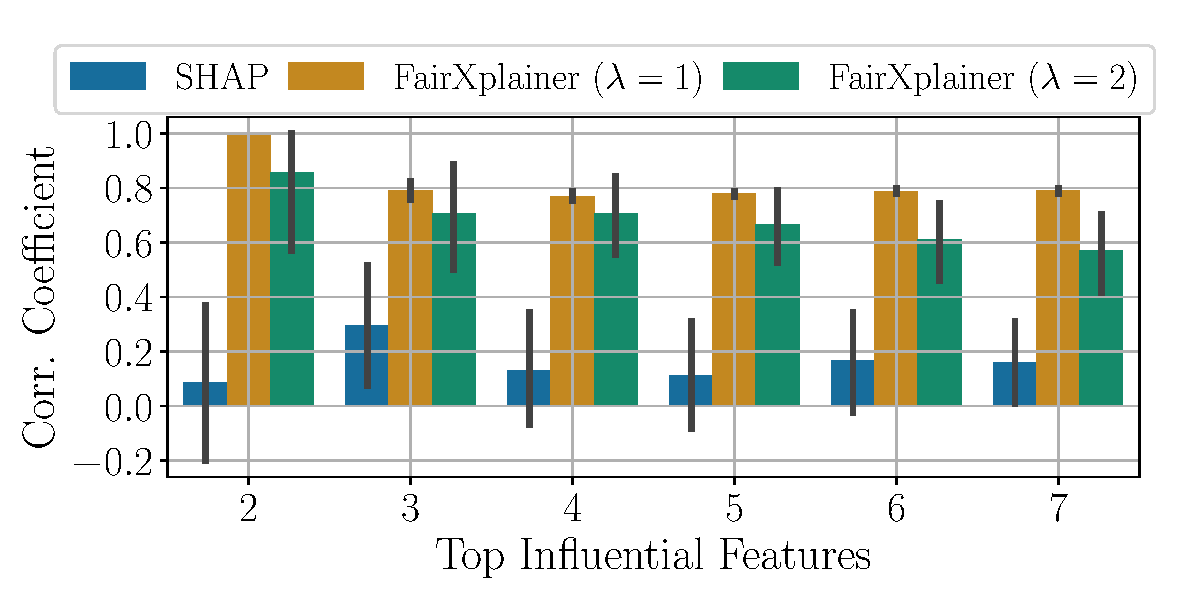
\includegraphics[scale=0.35]{figures/fairness/fif/intervention_adult_intersectional}}
	\caption{Results on fairness intervention on logistic regression classifiers for COMPAS and Adult datasets. Pearson's correlation coefficient between bias-difference due to the intervention and FIFs is higher for top ranked influential features by {\fairXplainer} compared to SHAP.}	
	\label{fairness_fairXplainer_fig:fairness_intervention_with_intersectional}
\end{figure}

\end{comment}



\begin{comment}


\begin{figure}
	\subfloat[{\fairXplainer} ($ \lambda = 1 $)]{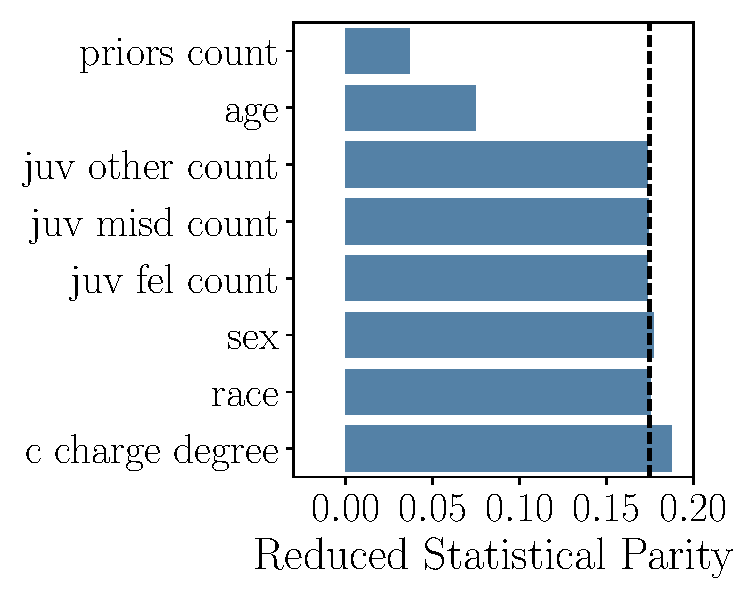
\includegraphics[scale=0.38]{figures/fairness/fif/intervention_individual}\label{fairness_fairXplainer_fig:intervention_individual}}
	\subfloat[{\fairXplainer} ($ \lambda = 2 $)]{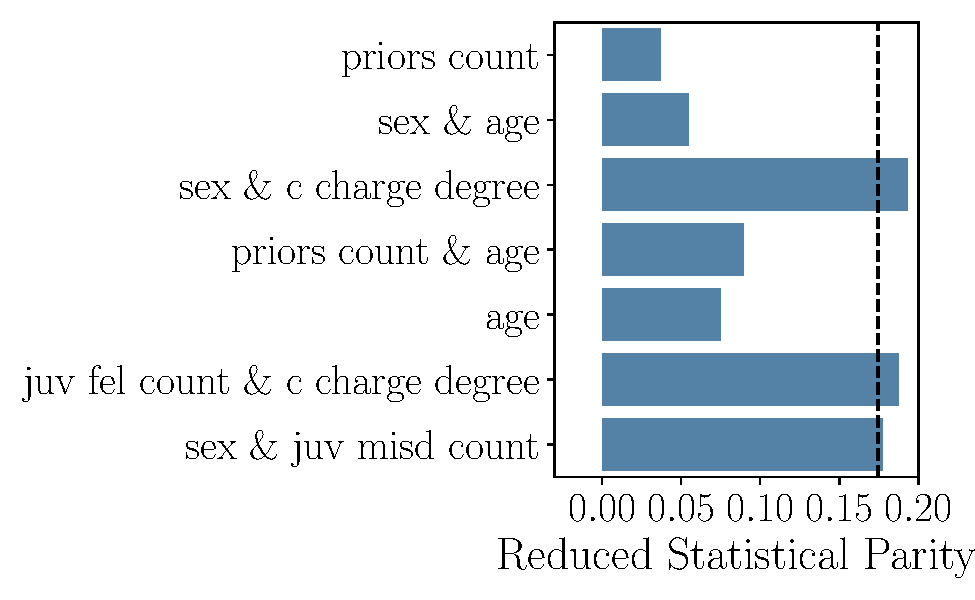
\includegraphics[scale=0.38]{figures/fairness/fif/intervention_intersectional}\label{fairness_fairXplainer_fig:intervention_intersectional}}
	\caption{\red{[In Appendix]} Intervention results. \red{Diff with QII, Yair ZIck's paper: data vs classifier intervention.}}
\end{figure}

\end{comment}
